%!TEX encoding = UTF-8 Unicode

\documentclass{hnuthesis}

% \usepackage{subfigure}
\usepackage{amsmath}
\usepackage{algorithmicx,algpseudocode}
\usepackage{float}
\usepackage{siunitx,amsmath,mathpazo,caption,subfig,multirow,makecell,booktabs,rotating,adjustbox}
\usepackage{afterpage}
\usepackage{notoccite}

\newcommand\blankpage{%
    \null
    \thispagestyle{empty}%
    \addtocounter{page}{-1}%
    \newpage}

% 学校代码
\hnucode{10532}
% 学校名称
\hnuname{湖南大学}
\enhnuname{Hunan University}
% 中图分类号
\clc{TP391}
% 密级
\secrettext{普通}

% 标题
\title{使用随机像素空间扰动的对抗样本检测}
\entitle{Adversarial Examples Detection Using Random Pixel-Space Perturbation}
% 作者
\author{Griveau Jordan}
\enauthor{Griveau Jordan}
% 学号
\authorid{LY2019093}
% 学院
\college{信息科学与工程学院}
% 专业
\major{计算机科学与技术}
\enmajor{Computer Science and Technology}
%学士学位获得学校,年份
\enmaster{Master of Science}
% 研究方向
\workon{第三类永动机}
% 导师
\supervisor{Professor JIANG Bin}
\ensupervisor{Professor JIANG Bin}
% 论文提交、答辩日期
\submitdate{2022年3月27日}
\defensedate{2022年--月--日}
\endate{March, 2022}
% 答辩委员会主席
\chair{待定}

\begin{document}
% 封面、原创性声明
\maketitle


\vspace*{0.2\textheight}

{\itshape Live as if you were to die tomorrow. Learn as if you
    were to live forever.}\bigbreak

\hfill Mahatma Gandhi
\afterpage{\blankpage}

% 摘要
\begin{abstract}
	\large
	与其他机器学习算法一样,神经网络很容易受到对抗性示例的影响,即包含特制扰
	动的输入,其唯一目的是欺骗网络进行错误分类。另一方面,由于对神经网络架构
	的改进,众所周知,它们对输入中的随机扰动更加稳健。这种对随机扰动的鲁棒性
	促使我提出了一种易于部署的对抗样本检测方法,该方法可以测量将随机噪声应用
	于输入图像之前和之后的预测不一致性。在三个流行基准 (Dogs vs.
	Cats、CIFAR-10 和 ImageNet) 的子集上评估该方法表明,它在针对更高分辨率图
	像的各种攻击中实现了高对抗样本检测性能。我的方法的主要优点是简单,计算成
	本低,并且不需要任何关于所使用攻击的先验知识,这使得我的方法很容易集成到
	其他防御框架中.

	我提出了一种检测对抗样本的新方法,该方法基于在输入上故意引入不同强度的高
	斯噪声。然后,计算两个分数,以评估模型在应用噪声之前和之后在不同强度下的预测差
	异。这种方法的优点是检测效率不依赖于关于所使用攻击的先验知识,因此可以应用于广泛
	的攻击和不同的对抗性扰动预算。此外,与最先进的防御或检测方法相反,我的方法对计算
	的要求很低,因为不需要对模型参数进行训练或优化。最后,此方法可以与其他检测方法结
	合使用,以提高整体应用程序的性能。我提出的方法是在研究了将加性高斯噪声应用于正常
	图像和对抗样本的影响并观察到据我所知并且在这项工作时尚未在之前的工作中讨论过的差
	异之后出现的。
	\keywords{深度学习;计算机视觉;对抗性例子}
\end{abstract}
\afterpage{\blankpage}

\begin{enabstract}
	\large
	Like other machine learning algorithms, neural networks have been vulnerable
	to adversarial examples, \emph{i.e.}, inputs containing specifically crafted
	perturbations whose only objective is to fool a network into
	misclassification. On the other hand, because of the improvements made on
	neural network architectures, they are known to be much more robust to
	random perturbations in the input. This robustness to random perturbations
	motivated me to propose an easy-to-deploy adversarial example detection
	method that measures prediction inconsistencies before and after applying
	random noise to an input image. Evaluating the method on subsets of three
	popular benchmarks (Dogs vs. Cats, CIFAR-10, and ImageNet) shows that it
	achieves high adversarial example detection performance for various attacks
	on higher resolution images. The main advantages of my approach are its
	simplicity, low computational cost, and the fact that it does not require
	any prior knowledge of the attack used, which makes it easy to integrate my
	method into other defense frameworks.
	\enkeywords{Deep Learning; Computer Vision; Adversarial Examples}
\end{enabstract}
\afterpage{\blankpage}

% 目录
\tableofcontents
% 插图附表索引
\listoffigures
\listoftables

% 正文章节
\mainmatter
\chapter{Introduction}
\label{Introduction}

\section{Motivation}
\begin{figure}[ht]
    \centering
    \subfloat[\centering]{{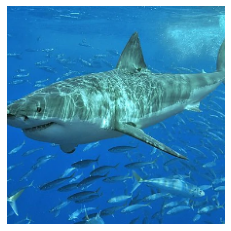
\includegraphics[width=.33\linewidth]{figures/intro/normal.png}}} %
    \subfloat[\centering]{{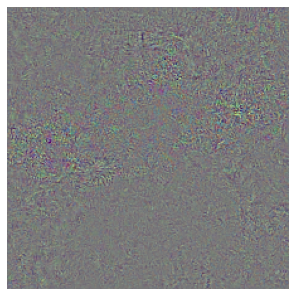
\includegraphics[width=.33\linewidth]{figures/intro/ae_diff.png}}} %
    \subfloat[\centering]{{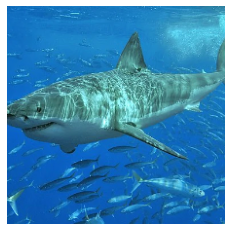
\includegraphics[width=.33\linewidth]{figures/intro/ae.png}}} %
    \caption{Normal image (A), adversarial perturbation (B), adversarial
        example (C). The model accurately classifies the normal image as a
        "white shark" while misclassifying the adversarial example as a "prairie
        chicken."}
    \label{fig:adversarial_examples}
\end{figure}

Deep neural networks (DNNs) have succeeded on numerous tasks, from image and
speech recognition (\cite{russakovsky_imagenet_2015,amodei_deep_2015}) to
self-driving cars (\cite{bojarski_end_2016}) and beating the world champion at
the game of Go (\cite{silver_mastering_2016}). However, despite achieving
state-of-the-art performance in various domains, \cite{szegedy_intriguing_2014}
showed that deep neural networks are vulnerable to adversarial examples,
\emph{i.e.}, inputs containing a carefully crafted perturbation that causes an
image classification model to make the wrong predictions. Researchers
demonstrated this phenomenon to be observable in computer vision and speech
recognition when \cite{carlini_audio_2018} showed that a perturbed audio
waveform could make a speech-to-text model drastically change the transcription,
as seen in figure \ref{fig:carlini_audio}.
\begin{figure}[ht]
    \centering
    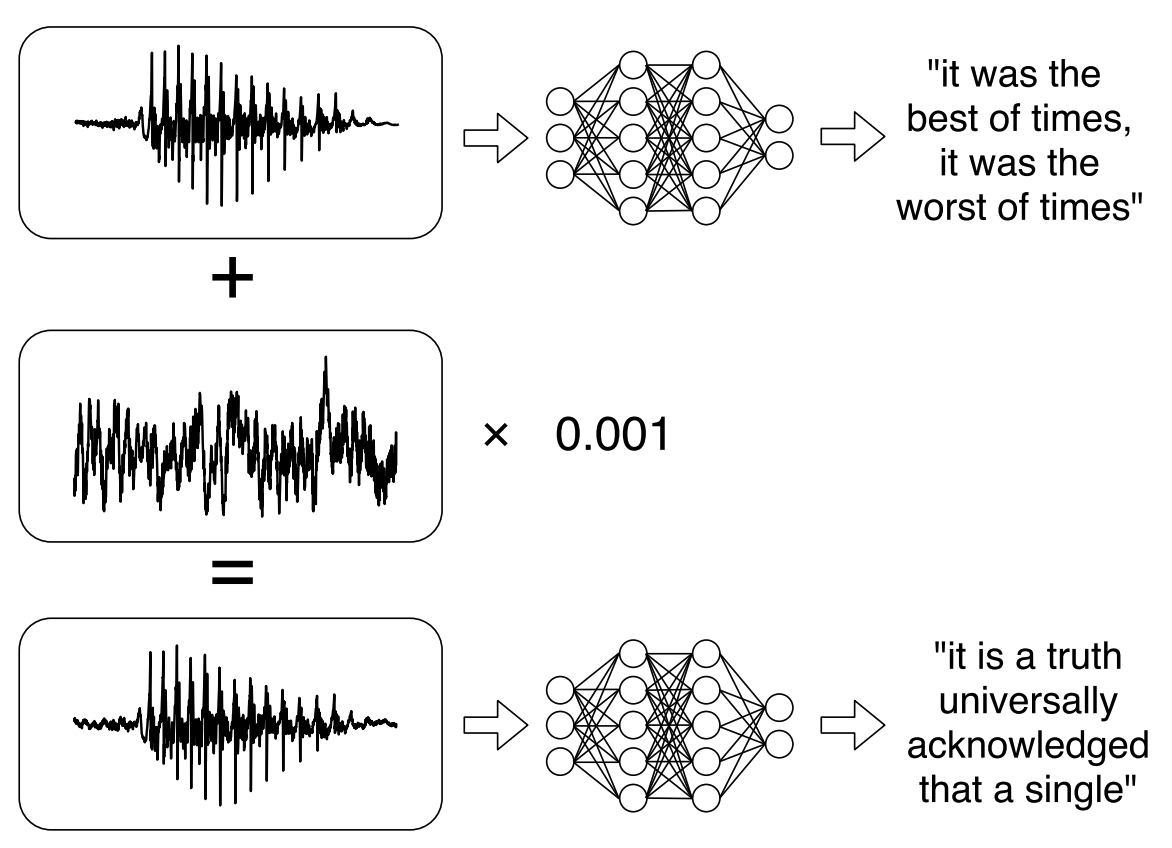
\includegraphics[width=.8\linewidth]{Figures/intro/carlini_noise.png}
    \caption{ Unnoticeable audio waveform added to an audio recording changes
        the transcription by the model drastically, by
        \cite{carlini_audio_2018}.}
    \label{fig:carlini_audio}
\end{figure}

One surprising aspect of these adversarial examples is that, as seen in figure
\ref{fig:noise}, the perturbation needed to fool a model into misclassification
can be so small that it is unnoticeable to a human observer. \cite{su_one_2019}
even demonstrated in a recent study that modifying a single pixel from the input
vector can be enough to fool a neural network, as shown in figure
\ref{fig:su_one_pixel}.

\begin{figure}[ht]
    \centering
    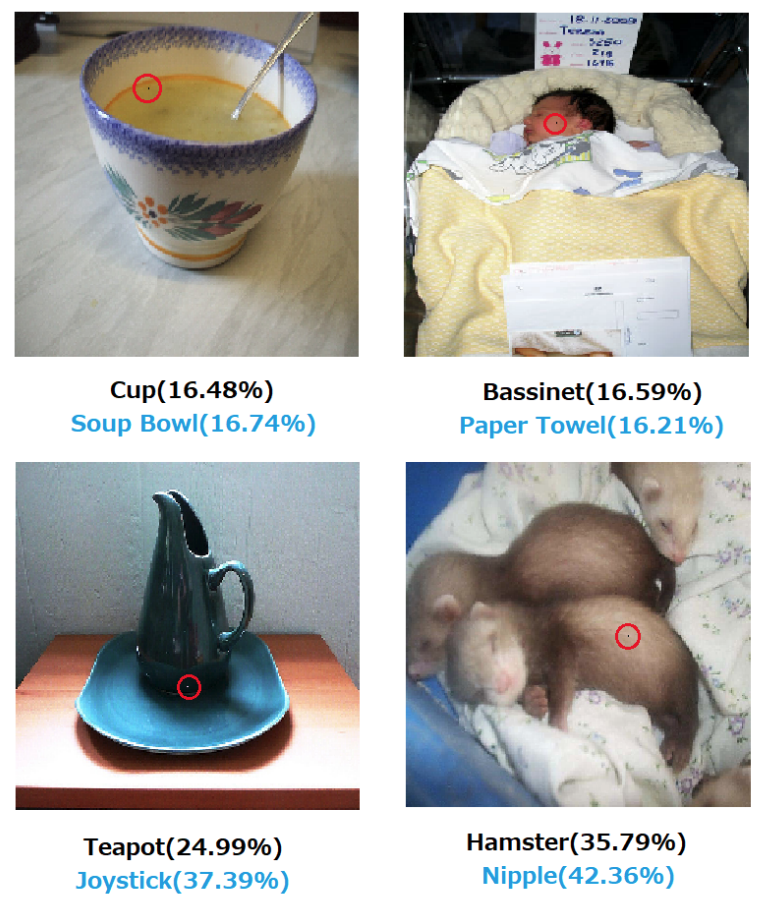
\includegraphics[width=.8\linewidth]{Figures/intro/su_one_pixel.png}
    \caption{ One-pixel attack by \cite{su_one_2019}. Modified pixels are
        circled in red. Original predictions in black and predictions with
        modified pixels in blue.}
    \label{fig:su_one_pixel}
\end{figure}

\begin{figure}[ht]
    \subfloat[]{%
        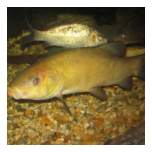
\includegraphics[clip,width=.33\linewidth]{Figures/fig2/Fig2a.png}%
    } \subfloat[]{%
        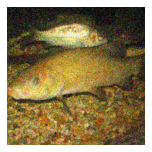
\includegraphics[clip,width=.33\linewidth]{Figures/fig2/Fig2b.png}%
    } \subfloat[]{%
        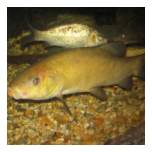
\includegraphics[clip,width=.33\linewidth]{Figures/fig2/Fig2c.png}%
    }

    \caption{ Normal image (A), noisy image (B), adversarial example (C). The
        model accurately predicts both the normal image and noisy image but
        misclassifies the adversarial example, despite the adversarial
        perturbation being $\approx{20}$ times smaller than the random
        perturbation in that case. }
    \label{fig:noise}
\end{figure}

On the other hand, with the constant improvement of neural network
architectures, (\cite{he_deep_2015,vaswani_attention_2017,huang_densely_2018})
and regularization techniques such as dropout by \cite{srivastava_dropout_2014},
neural networks have become more and more robust against randomly perturbed
inputs as demonstrated by \cite{hendrycks_benchmarking_2019}. Thus, as long as
the random perturbations are not too significant, \emph{e.g.}, rotation of the
image, compression deterioration (\emph{e.g.}, JPEG), brightness or contrast
shift, the neural network will still accurately predict the images.

This divergence of robustness displayed by neural networks when facing random
and adversarial perturbations motivated me to experiment with the robustness of
adversarial examples themselves by intentionally adding a random perturbation on
these modified samples.


\section{Main Contribution}
I propose a novel method for detecting adversarial examples based on
intentionally introducing Gaussian noise on the input with varying intensity.
Then, two scores are computed that evaluate the difference of prediction by the
model before applying noise and after, at varying intensity. The advantage of
this method is that the detection efficacy does not rely on prior knowledge
about the attack used and thus can be applied over a wide range of attacks and
at varying adversarial perturbation budgets.

Furthermore, contrary to state-of-the-art defense or detection approaches, my
method is computationally low demanding because no training or optimization of
the model parameters is required.

Lastly, this method can be combined with other detection methods to increase the
overall application's performance. The method I propose emerged after studying
the effects of applying additive Gaussian noise to normal images and adversarial
examples and observing a disparity that, to the best of my knowledge and at the
time of this work, has not been discussed in prior work.


\section{Thesis Structure}
The material described in chapter \ref{RelatedWork} first provides a brief
explanation and general knowledge about neural networks and the different parts
they contain. Then it includes a description of adversarial examples, the
dangers they represent, and the background knowledge needed to generate them,
using different methods emerging from the research community.

Chapter \ref{Experiments} introduces the experiments I conducted and some of the
results that motivated me to pursue and propose the methodology I later present
and describe in chapter \ref{Methodology} which includes the detection
performances.

\chapter{Related Work}
\label{RelatedWork}
\section{Neural Networks}
\label{neural_networks}

\overridetextsize
Artificial Intelligence (A.I.), Deep Learning, and Machine Learning have become
buzzwords in recent years, with media, movies, and the general public often
romanticizing and sometimes even humanizing A.I.s. However, what propelled this
enthusiasm is rooted in reality. More recent achievements and revolutions made
in multiple domains with the help of neural networks, even if not rivaling human
capabilities in most scenarios, have been consequent.

The enthusiasm of the general public and scientific community in artificial
intelligence is relatively recent; however, this idea of artificially mimicking
the human brain (seen in figure \ref{fig:biological_neuron}) dates back almost a
century, when a neurophysiologist and a mathematician proposed the first
mathematical model of a neuron (see figure \ref{fig:mccullock_neuron}) called
the McCulloch-Pitts Neuron \cite{warren_s_mcculloch_walter_pitts_logical_1943}.

\begin{figure}[ht]
    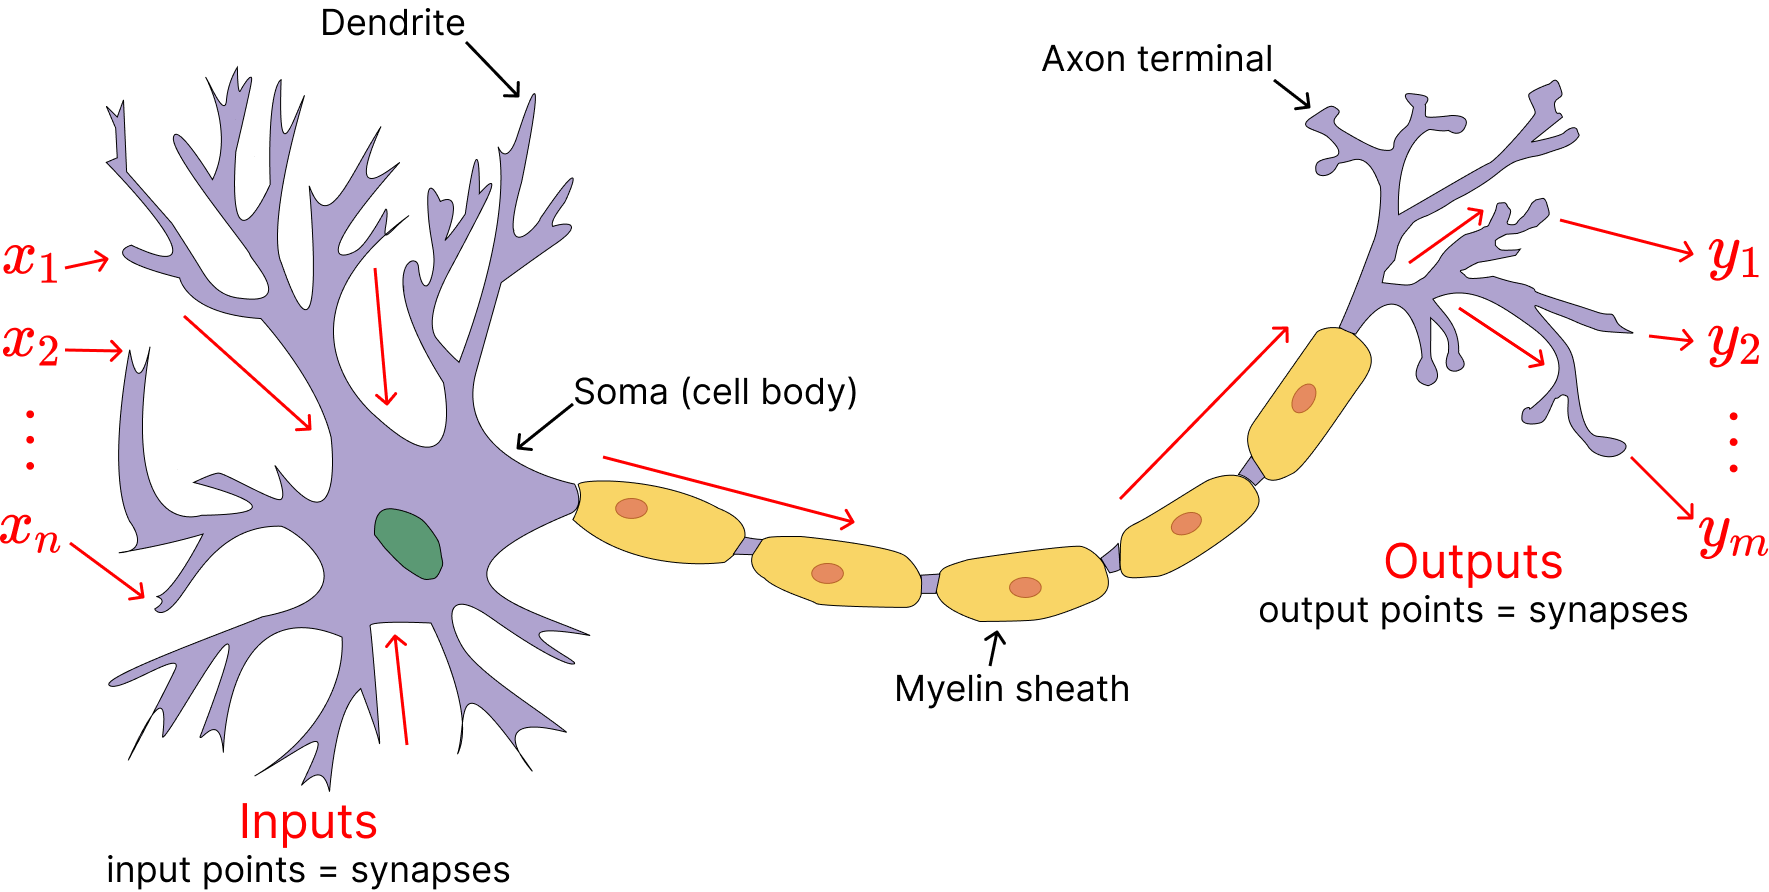
\includegraphics[clip,width=1\columnwidth]{Figures/related/biological_neuron.png}
    \caption{ Representation of a biological neuron. }
    \label{fig:biological_neuron}
\end{figure}

\begin{figure}[htp]
    \centering
    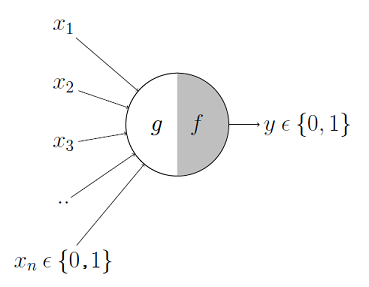
\includegraphics[clip,width=.5\columnwidth]{Figures/related/cullock-neuron.png}
    \caption{ McCulloch-Pitts Neuron, first mathematical model of a neuron. }
    \label{fig:mccullock_neuron}
\end{figure}

Fifteen years later, a psychologist used the McCulloch-Pitts Neuron, where he
proposed the Mark I Perceptron \cite{brain_perceptron_1958}. The breakthrough
proposed by Rosenblatt was that the network could learn by modifying the
neurons' weights through successively passed inputs to minimize the difference
between the desired output and the actual output.

During the next few decades, the field saw some minor improvements, but the
delivery and actual real-world use of A.I.s was minimal, if not nonexistent, and
could not live up to the buildup displayed in media, even at that time. Finally,
\cite{minsky_perceptrons_1969} published a book that laid out problems with
neural networks, notably with their conclusion on the perceptron proposed by
Rosenblatt, stating that this approach could not be translated into
multi-layered neural networks, as the computational cost to evaluate each
layers' neurons would be astronomic. This book, among others, started the era of
"A.I. winter," a period of reduced funding and interest in artificial
intelligence research.

The interest and enthusiasm for neural networks rallied in the nineties with the
rediscoveries of the components that now form the pillar of today's neural
networks: Backprogration and Gradient Descent.


\paragraph{Neural networks,} also known as artificial neural networks (ANNs),
are a subset of machine learning and are at the heart of deep learning
algorithms. Their name and structure are inspired by the human brain, mimicking
the way that biological neurons (see fig. \ref{fig:biological_neuron}) signal to
one another.

Artificial neural networks are thus, similarly to the human brain, comprised of
multiple layers of artificial neurons (see fig. \ref{fig:artificial_neuron} and
fig. \ref{fig:fcnn}).

\begin{figure}[ht]
    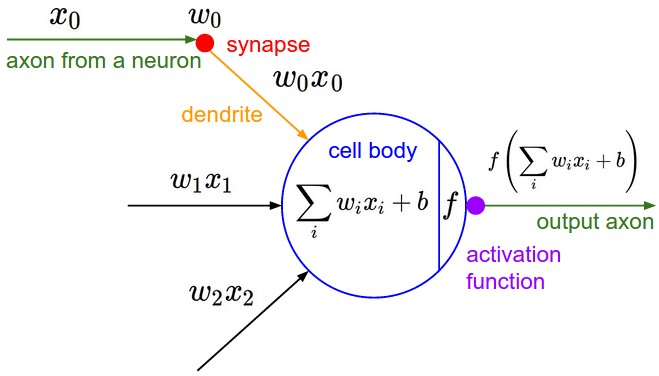
\includegraphics[clip,width=1\columnwidth]{Figures/related/artificial_neuron.jpeg}
    \caption{ Representation of an artificial Neuron. }
    \label{fig:artificial_neuron}
\end{figure}

\begin{figure}[t]
    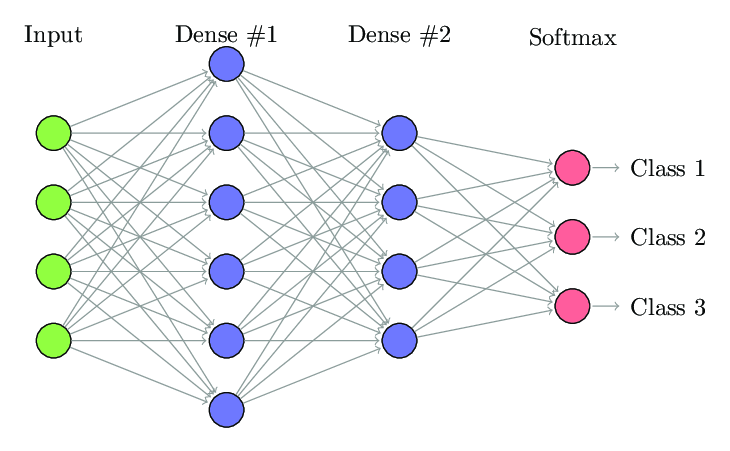
\includegraphics[clip,width=1\columnwidth]{Figures/related/fcnn.png}
    \caption{ Fully connected neural network containing two hidden layers. }
    \label{fig:fcnn}
\end{figure}

% https://www.oreilly.com/library/view/tensorflow-for-deep/9781491980446/ch04.html

Figure \ref{fig:fcnn} represents a simple neural network architecture with two
hidden fully connected layers between the input and output layer. Each hidden
layer contains an arbitrary number of artificial neurons that are fully
connected to the next layer of neurons. The input layer contains several nodes
(or neurons) equal to the dimension of the input. For example, if using a black
and white image of 24 pixels, the input layer would contain $24 \times 24$
nodes. As for the output layer, the number of nodes represents the number of
classes. This type of architecture is widely used. Their primary advantage is
that they are structure agnostic, \emph{i.e.,} no particular assumptions need to
be made about the input.

% https://andrew.gibiansky.com/blog/machine-learning/fully-connected-neural-networks/
Mathematically, we can represent the network shown in figure \ref{fig:fcnn}.

Let $x \in \mathbf{R}$ represents the input. Then, we can perform forward
propagation as follows:

Let $a^{[1]}$ represent the first hidden layer and $a^{[1]}_{i}$ represent
$a^{[1]}$'s $i_{th}$ node:
\begin{equation} \label{eq:fcnn_layer_1}
    A^{[1]} =
    \begin{cases}
        a^{[1]}_{1} = f(x_{1}w^{[1]}_{11} + x_{2}w^{[1]}_{21} + x_{3}w^{[1]}_{31} + x_{4}w^{[1]}_{41} + b^{[1]}_{1}) \\
        a^{[1]}_{2} = f(x_{1}w^{[1]}_{12} + x_{2}w^{[1]}_{22} + x_{3}w^{[1]}_{32} + x_{4}w^{[1]}_{42} + b^{[1]}_{2}) \\
        a^{[1]}_{3} = f(x_{1}w^{[1]}_{13} + x_{2}w^{[1]}_{23} + x_{3}w^{[1]}_{33} + x_{4}w^{[1]}_{43} + b^{[1]}_{3}) \\
        a^{[1]}_{4} = f(x_{1}w^{[1]}_{14} + x_{2}w^{[1]}_{24} + x_{3}w^{[1]}_{34} + x_{4}w^{[1]}_{44} + b^{[1]}_{4}) \\
        a^{[1]}_{5} = f(x_{1}w^{[1]}_{15} + x_{2}w^{[1]}_{25} + x_{3}w^{[1]}_{35} + x_{4}w^{[1]}_{45} + b^{[1]}_{5}) \\
        a^{[1]}_{6} = f(x_{1}w^{[1]}_{16} + x_{2}w^{[1]}_{26} + x_{3}w^{[1]}_{36} + x_{4}w^{[1]}_{46} + b^{[1]}_{6})
    \end{cases}
    ,
\end{equation}
or in vectorized form:
\begin{equation} \label{eq:fcnn_layer_1_vec}
    A^{[1]} = f(W^{[1]} X + b^{[1]}),
\end{equation}
where $b^{[1]}$ represents the bias for the first hidden layer. Biases are
learnable (by the model) parameters used to shift the activation function
(explained next paragraph) right or left, in order to better fit to the data.

Then, from the first hidden layer to the second hidden layer:
\begin{equation} \label{eq:fcnn_layer_2_vec}
    A^{[2]} = f(W^{[2]} A^{[1]} + b^{[2]}),
\end{equation}
where we utilize the output of the previous layer $A^{[1]}$. We can observe the
simplicity of adding or removing a hidden layer from a fully-connected network.

Finally, we can compute the final layer of the network:
\begin{equation} \label{eq:fcnn_layer_last}
    \begin{cases}
        y_{1} = f(a^{[2]}_{1}w^{[3]}_{11} + a^{[2]}_{2}w^{[3]}_{21} + a^{[2]}_{3}w^{[3]}_{31} + a^{[2]}_{4}w^{[3]}_{41} + a^{[2]}_{5}w^{[3]}_{51} + a^{[2]}_{6}w^{[3]}_{61} + b^{[3]}_{1}) \\
        y_{2} = f(a^{[2]}_{2}w^{[3]}_{12} + a^{[2]}_{2}w^{[3]}_{22} + a^{[2]}_{3}w^{[3]}_{32} + a^{[2]}_{4}w^{[3]}_{42} + a^{[2]}_{5}w^{[3]}_{52} + a^{[2]}_{6}w^{[3]}_{62} + b^{[3]}_{2}) \\
        y_{3} = f(a^{[2]}_{3}w^{[3]}_{13} + a^{[2]}_{2}w^{[3]}_{23} + a^{[2]}_{3}w^{[3]}_{33} + a^{[2]}_{4}w^{[3]}_{43} + a^{[2]}_{5}w^{[3]}_{53} + a^{[2]}_{6}w^{[3]}_{63} + b^{[3]}_{3}) \\
    \end{cases}
    ,
\end{equation}
Alternatively, in the vectorized form:
\begin{equation} \label{eq:fcnn_layer_last_vec}
    Y = f(W^{[3]} A^{[2]} + b^{[3]}),
\end{equation}

In the previous equations (Eq. \ref{eq:fcnn_layer_1}, Eq.
\ref{eq:fcnn_layer_1_vec}, Eq. \ref{eq:fcnn_layer_2_vec}, Eq.
\ref{eq:fcnn_layer_last}, Eq. \ref{eq:fcnn_layer_last_vec}), $f$ represents a
nonlinear function, also called activation function. Activation functions act as
the \emph{axon} seen in figure \ref{fig:biological_neuron}. It takes in the
output signal from the previous neuron and converts it into the input for the
next neuron. These nonlinear functions add non-linearity to a neural network, as
their name implies.

\begin{figure}[htb]
    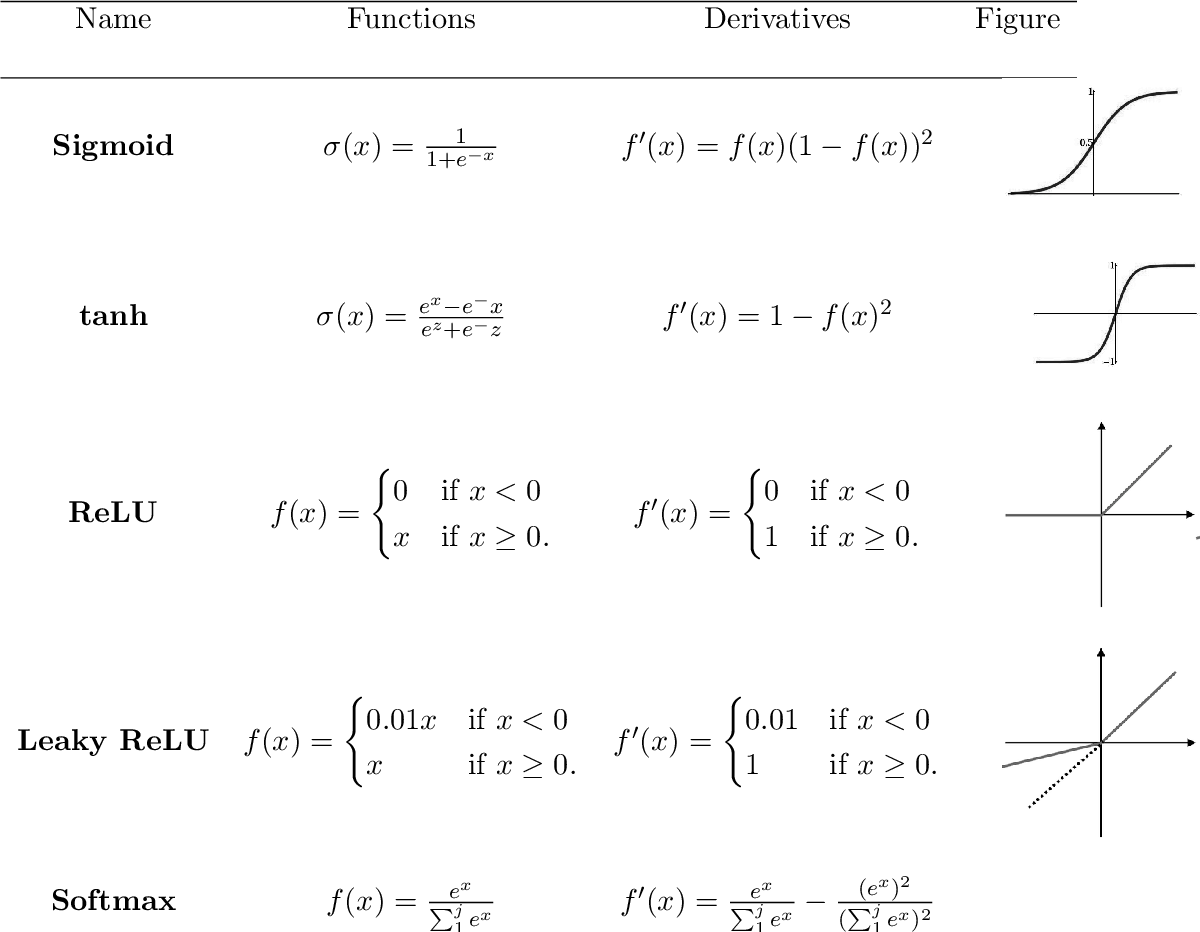
\includegraphics[clip,width=1\columnwidth]{Figures/related/activation_functions.png}
    \caption{ Widely used activation functions. }
    \label{fig:activation_functions}
\end{figure}

Figure \ref{fig:activation_functions} shows some of the widely used activation
functions used in neural networks. In our previous example, the final layer of
our fully connected neural networks contains three nodes (for three
classes); accordingly, this network architecture would be used for multi-class
classification problems. The activation function widely used for this type of
problem is the softmax function, seen in figure \ref{fig:activation_functions}),
where it's equation is:
\begin{equation} \label{eq:softmax}
    f(x) = \frac{e^{x}}{\sum^{j}_{i}e^{x}},
\end{equation}
where $x$ is the input, $j$ is the number of classes and $e$ is the standard
exponential function for output vector.


The softmax function outputs values in the range of 0 to 1. In our neural
network example from figure \ref{fig:fcnn}, with three output classes, the
model's output could be a vector such as: $[0.8, 0.1, 0.1]$. We can translate
this output as the model being 80\% confident about the input being the first
class and 10\% confident for the second and third class, respectively.

As for the hidden layers, a widespread activation is the rectified linear unit,
commonly referred to as ReLU:
\begin{equation} \label{eq:relu}
    f(x) =
    \begin{cases}
        0 \quad \textrm{if} \; x < 0 \\
        x \quad \textrm{if} \; x \geq 1
    \end{cases}
    ,
\end{equation}
or its modification Leaky ReLU:
\begin{equation} \label{eq:leaky_relu}
    f(x) =
    \begin{cases}
        0.01x \quad \textrm{if} \; x < 0 \\
        x \quad \quad \; \; \; \textrm{if} \; x \geq 1
    \end{cases}
    .
\end{equation}
We refer to passing the input through layer-by-layer like evoked beforehand as
"forward propagation." Forward propagation is one of the core processes needed
to train a neural network. Backpropagation \cite{rumelhart_learning_1986} is the
next step in this process, and it refers to the method of calculating the
gradient of the parameters of the neural network, i.e., weights and biases.
Inversely with forward propagation, this method traverses the network from the
output to the input to compute gradient with respect to some parameters. The
objective of updating these parameters is to minimize a chosen cost function.
For example, in our neural network example again, we could use the cross-entropy
function defined as:
\begin{equation} \label{eq:cross-entropy}
    -\sum^{3}_{c=1}y_{o,c} \log{(p_{o,c})},
\end{equation}
for a three-classes classification problem, where $y$ is a binary indicator if
class label $c$ is the correct classification for observation $o$ and $p$ is the
predicted probability that $o$ is of class $c$.

Forward propagation and backpropagation are alternatively used when training a
neural network and are interdependent: forward propagation computes and stores
intermediate variables and parameters, while backpropagation computes the
gradients of these same parameters. Training a network thus requires
considerably more memory than simply predicting a sample, as backpropagation
requires the intermediate values in order to be computed.

To recapitulate, a neural network can be written as a function $F(x)=y$, where
$x$ represents the input and $y$ represents the output. The final layer of a
neural network performing classification is often the softmax activation
function. Therefore, $F(x)$ outputs a probability distribution, where $F(x)_{i}$
represents the probability that input $x$ belongs to class $i$. We write the
final output of the layer as $F(x)=\textup{softmax}(Z(x))$, where $Z(x)$ is the
network output vector containing \textit{logits}, \emph{i.e.,} raw values before
the activation function. Finally, the classifier function that returns the most
likely class label can be written as $C(x)=\textup{argmax}_{i}{(F(x)_{i})}$.

\section{Convolutional Neural Networks}
\label{CNNs}
% https://paperswithcode.com/methods/category/convolutional-neural-networks

\begin{figure}[ht]
    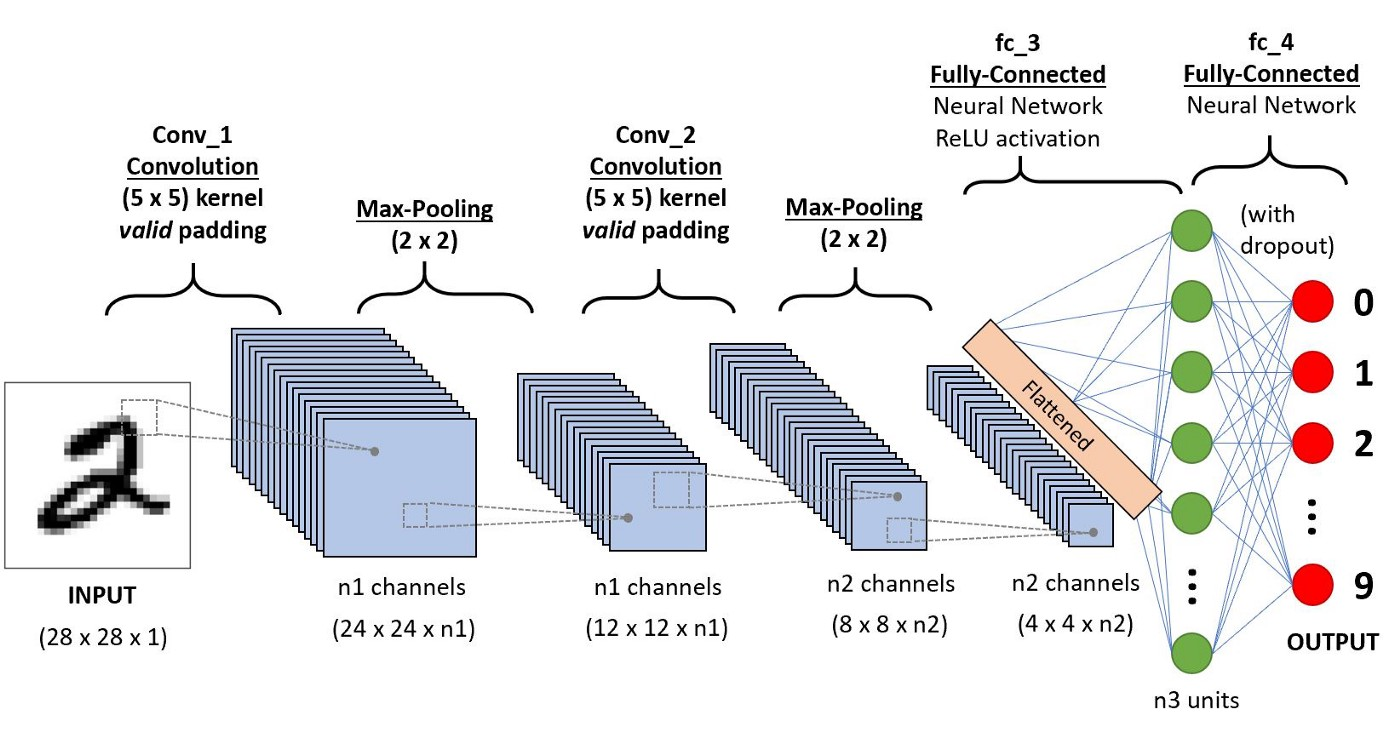
\includegraphics[clip,width=1\columnwidth]{Figures/related/cnn.jpeg}
    \caption{ Architecture of a classic convolutional neural network. }
    \label{fig:cnn}
\end{figure}

Convolutional neural networks (CNNs) \cite{lecun_object_1999}, similarly to the
neural network architectures discussed in the previous section
\ref{neural_networks} are a class of artificial neural networks. CNNs are
commonly used in computer vision to extract features from images or videos and
have been shown to work exceptionally well for this type of data. They are
similarly composed of layers of neurons with learnable parameters, \emph{i.e.,}
weights and biases. The main difference with the more traditional architectures
is that convolutional neural networks make the explicit assumption that the
inputs are of image-type, \emph{i.e.,} images or videos.

The problem with regular neural networks, when applied to images, is that the
fully-connected layers in these architectures do not scale well with this type
of input: a color image of size $224 \times 224$ would represent $150.000$
weights ($224 \times 224 \times 3$), which would quickly result in a costly and
inefficient model. In convolutional neural networks, the neurons are
three-dimensional: width, height, and depth (number of channels: red, green,
blue). These convolutional layers can drastically reduce the number of
parameters, thus the model's size.



Convolutional neural networks, or ConvNets, transform the input image into the
final output vector containing a score for each class through a sequence of
layers. Figure \ref{fig:cnn} shows an example architecture for a convolutional
neural network performing multi-class classification on black and white $28
    \times 28$ images of digits from 0 to 9.

This architecture comports:
\begin{itemize}
    \item Two convolutional layers: the core building block of any ConvNet. Both
          layers contain multiple filters (also called kernels) of size $5
              \times 5$. As seen in figure \ref{fig:kernels}, filters learn visual
          features: the earlier filters, \emph{i.e.,} the ones present at
          shallow depth, learn more basic features. In contrast, filters at the
          last layers learn more complex ones, as seen in figure
          \ref{fig:kernels_5}, since they are combinations of all the previous
          layer's filters.
          \begin{figure}[ht]
              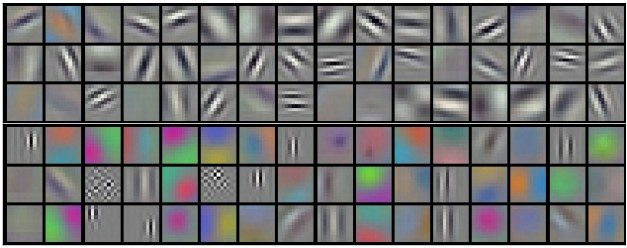
\includegraphics[clip,width=1\columnwidth]{Figures/related/kernels.jpeg}
              \caption{ $11 \times 11 \times 3$ filters learned by the first convolutional
                  layer on $224 \times 224 \times 3$ input images, experiment by
                  \cite{krizhevsky_imagenet_2017-1}. }
              \label{fig:kernels}
          \end{figure}
    \item Pooling layers: these layers will perform a down-sampling operation
          along the spatial dimensions, \emph{e.g.,} width and height. The
          primary function of a pooling layer is to reduce the spatial size of
          the representation, to reduce the number of parameters, thus reducing
          the computation cost of the model.
    \item Fully connected layers: as seen in the previous section
          \ref{neural_networks}. Since neurons from convolutional layers are
          multidimensional, their results need to be flattened before being fed
          into fully-connected layers. This last layer, similarly to ANNs seen
          previously, will output a probability vector containing the score for
          each class.
\end{itemize}



\begin{figure}[htp]
    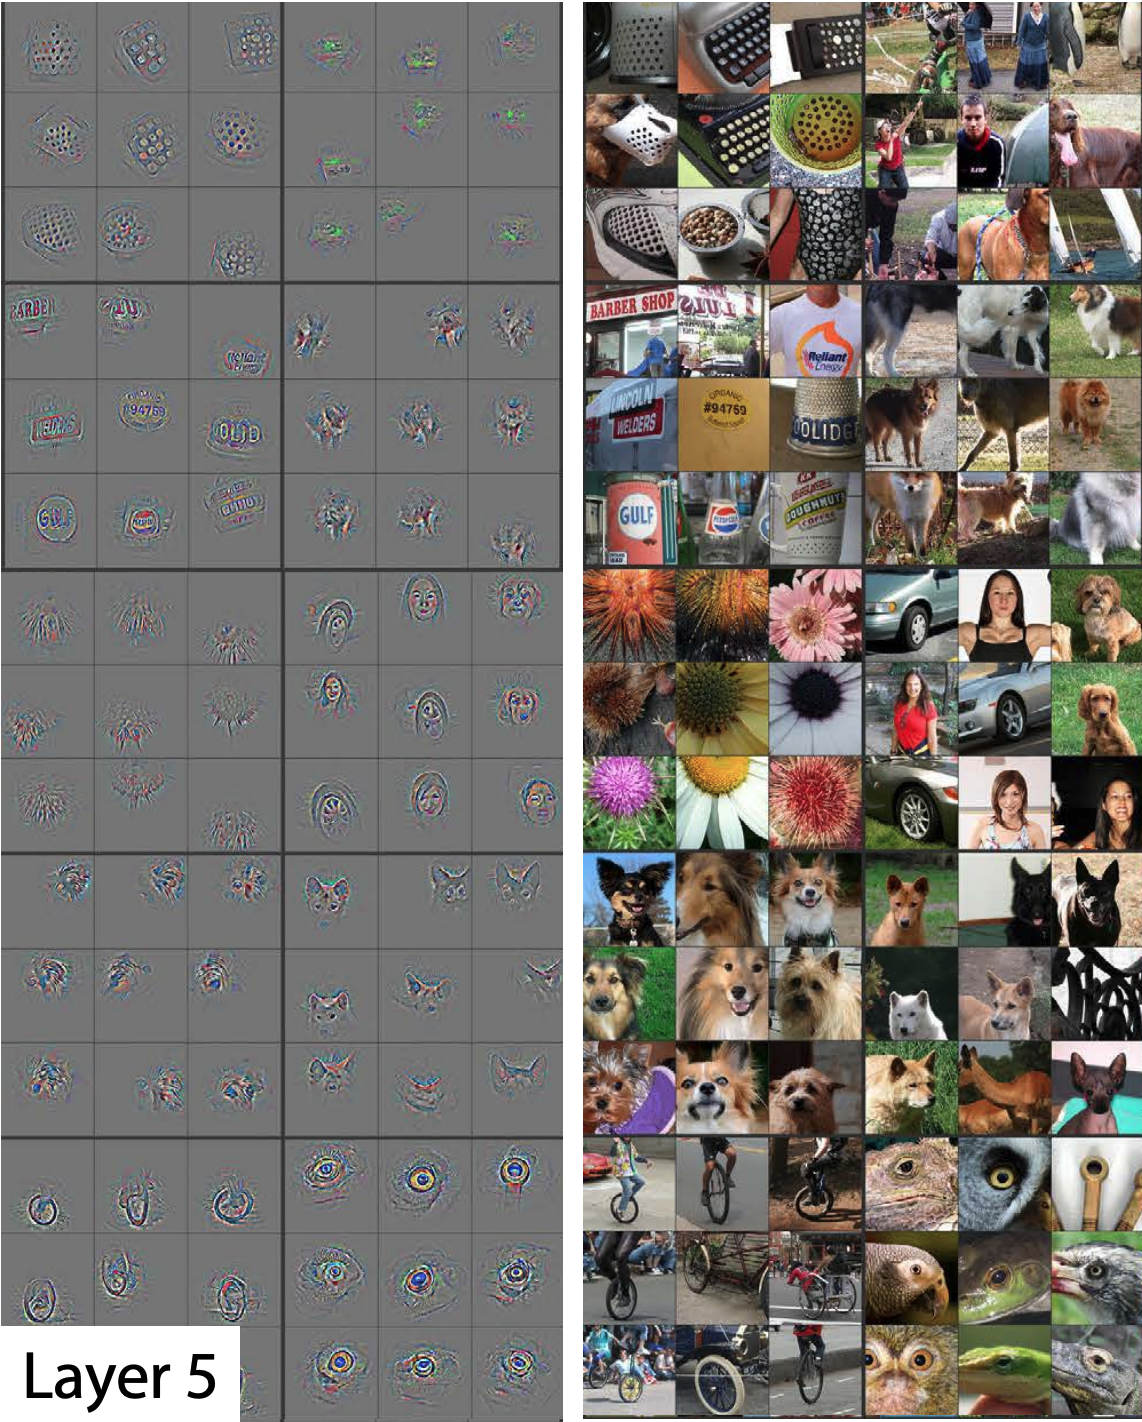
\includegraphics[clip,width=1\columnwidth]{Figures/related/kernels_5.png}
    \caption{ Filters learned by the fifth convolutional layer, experiment by
        \cite{zeiler_visualizing_2013}. }
    \label{fig:kernels_5}
\end{figure}

In short, convolutional neural networks are artificial networks that contain
convolutional layers. These architectures perform exceptionally well on
image-based data with the added benefit of fewer parameters compared to more
traditional ANNs.


In this work, since the entirety of my research is conducted on images,
convolutional neural networks are the only type of architecture that I consider.

\section{Adversarial Examples}
\label{Adversarial_examples}

As seen with figure \ref{fig:adversarial_examples}, adversarial examples are
samples that contain intentional feature modifications that cause a model to
misclassify the sample, \emph{e.g.} an image of a "shark" being misclassified as
a "bee" after adding an invisible (for a human observer) modification to the
image.

A neural network classifying an image of a shark as a bee may only seem comical
and not particularly problematic. However, with the rapidly growing usage of
neural networks in real-world applications, we need to have the certitude that
the models in use will not be as trivially fooled.

\begin{figure}[b]
    \centering
    \subfloat[]{%
        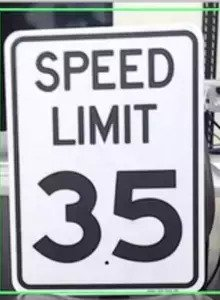
\includegraphics[clip,width=.33\linewidth]{Figures/related/artificial_examples/7.jpeg}%
    } \subfloat[]{%
        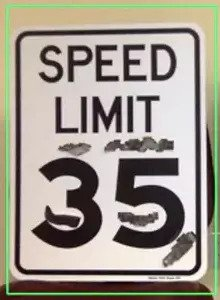
\includegraphics[clip,width=.33\linewidth]{Figures/related/artificial_examples/10.jpeg}%
    } \subfloat[]{%
        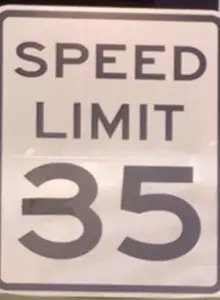
\includegraphics[clip,width=.33\linewidth]{Figures/related/artificial_examples/17.jpeg}%
    } \caption{Speed limit signs modified (B, C) that fools the Tesla model X
        and S (model 2016). (B) is identified as a 45-mph sign, while (C) is
        identified as a 85-mph speed sign.}
    \label{fig:mcafee_tesla}
\end{figure}

Recently, McAfee Advanced Threat Research researchers experimented with
adversarial examples in a physical context (\cite{noauthor_model_2020}). They
physically applied modifications to road speed signs in order for a Tesla car to
misidentify the signs. Figure \ref{fig:mcafee_tesla} shows the original 35-mph
road sign (A) as well as two of the physical adversarial examples they created
(B, C). (A) is accurately identified with a 95.93\% confidence, while (B) is
wrongly identified as a 45-mph sign with 99.88\% confidence, and (C) is also
wrongly identified, but as an 85-mph sign! In this context, it is easy to
imagine why and how this can be a problem that needs to be addressed.




With the ever-growing research on the vulnerability of NNs, there are now many
different methods to generate adversarial examples. The common objective of such
methods is to, from a normal image $x$, create a perturbation $\delta$ and add
it to the original image so that the new sample $x^{\prime}=x+\delta$ is
misclassified by a model. We refer to a sample that fulfills this objective as
an \textit{untargeted} adversarial example.

On the contrary, a \textit{targeted} adversarial example $x^{\prime}$ is
designed to be classified by a model as a specified target class $t$. As a
result, targeted adversarial examples are typically more challenging to produce
and may require a more significant perturbation than untargeted attacks.

We can thus formulate the optimization problem to craft adversarial examples as:
\begin{equation} \label{eq:adversarial_example_min}
    \min_{x}D(x+\delta),
\end{equation}


such that the classification $C(x^\prime)\neq{y}$ for an untargeted attack,
where $y$ is the actual class of the input, or $C(x^\prime)={t}$ for a targeted
attack, where $t$ is the targeted class.

$D$ represents a distance metric, usually, $p$-norm defined as:
\begin{equation} \label{eq:p-norm}
    \lVert D
    \lVert_{p}=\left(\sum_{i=1}^{n}|d|^{p}\right)^{\frac{1}{p}}.
\end{equation}

The remainder of this section contains a brief explanation of some of the
popular methods used to generate adversarial examples.

\paragraph{Fast Gradient Sign Method (FGSM).}
Ian Goodfellow \emph{et al} first introduced a method for crafting adversarial examples
\cite{goodfellow_explaining_2015} against GoogLeNet \cite{szegedy_going_2014}.
To generate an adversarial sample $x^{\prime}$ that maximizes the objective $J$,
FGSM uses the gradients of the cost function with respect to the normal input
image $x$:
\begin{align} \label{eq:fgsm} x^{\prime}=x+\epsilon
    sign\left(\nabla_{x}J\left(\Theta,x,y\right)\right),\end{align} where the
multiplier $\epsilon$ is used to ensure that the perturbation is kept small, and
$\Theta$ represents the parameters of the model.

\paragraph{Basic Iterative Method (BIM).}
Alexey Kurakin \emph{et al} proposed an extension of the Fast Gradient Sign Method
\cite{kurakin_adversarial_2017}. Rather than generating the adversarial sample
in one step, BIM applies adversarial noise multiple times with a step size
$\alpha$. The benefit of iteratively crafting the adversarial sample
$x^{\prime}$ is that intermediate results can be clipped at each step to ensure
that the generated samples are within an $\epsilon$ distance to the original
input $x$:
\begin{align} \label{eq:bim}
    x^{\prime}_{n+1}=clip_{x,\epsilon}
    \left\{ x^{\prime}_{n}+\alpha.sign\left(\nabla_{x}J\left(x^{\prime}_{n},y\right)\right)\right\},
\end{align}
where $x^{\prime}_{0}=x$.

\paragraph{Carlini \& Wagner (CW).}
Nicholas Carlini and David Wagner proposed a powerful method to generate
adversarial examples \cite{carlini_towards_2017} that can defeat the defensive
distillation approach published by Nicolas Papernot \emph{et al}
\cite{papernot_distillation_2016}. In their paper, the authors construct an
attack for: $L_{0}$, $L_{2}$ and $L_{\infty}$ distance metrics.

In my experiments, I use the attack that seeks low distortion in the $L_{2}$
distance metric. The final optimization problem for the CW $L_{2}$ attack can be
defined as
\begin{align} \label{eq:cw_min}
    \min{\lVert x^{\prime}-x\lVert_{2}^{2}+c\cdot\ell(x^{\prime})},
\end{align}
where $c$ is a constant chosen via binary search that determine the success
probability of the attack. The loss function $\ell$ is the best among seven
evaluated by the authors, written as
\begin{align} \label{eq:cw_lf}
    \ell(x^{\prime})=\max{\left(\max{\left\{ Z(x^{\prime})_{i}:i\neq t\right\} }-Z(x^{\prime})_{t},-k\right)},
\end{align}
where $-k$ is a parameter to specify how confident we want the adversarial
example to be classified as $t$ by the model.

The CW method is a state-of-the-art attack and effectively finds adversarial
examples with a small perturbation size. However, this method is computationally
expensive to run.

\paragraph{Decoupled Direction and Norm (DDN).}
Jérôme Rony \emph{et al} proposed an improvement over the CW method
\cite{rony_decoupling_2019}. The DDN method can obtain comparable results in
terms of perturbation size but with considerably fewer iterations. At each
iteration $k$, refine noise $\beta_{k}$ by considering a larger norm
$\epsilon_{k+1}=(1+\gamma)\epsilon_{k}$ or smaller norm
$\epsilon_{k+1}=(1-\gamma)\epsilon_{k}$ depending on if $x+\beta_{k}$ is
adversarial or not. Finally, the method returns the clipped adversarial sample
that has the lowest $L_{2}$-norm.

Figure \ref{fig:samples_ae} shows three samples generated using the basic
iterative method (B), decoupled direction and norm (D), and the Carlini \&
Wagner method (F). The model correctly predicts the natural image (A) as an
image of a church while predicting the generated samples as images of chickens.
The perturbation size for each sample is: $L_2 \approx 2.00$ for the BIM sample
(B), $L_2 \approx 1.40$ for the DDN (D) sample and $L_2 \approx 1.37$ for the CW
sample. As discussed earlier, DDN and CW methods can generate samples with a
smaller perturbation than methods such as BIM or FGSM.

\begin{figure}[htb]
    \centering
    \begin{tabular}{@{}cc@{}} \multicolumn{2}{c}{
            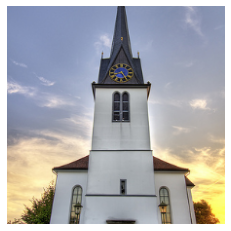
\includegraphics[width=.25\columnwidth]{Figures/related/attacks/original.png}
        }                       \\
        \multicolumn{2}{c}{ (A) Original image }
        \\
        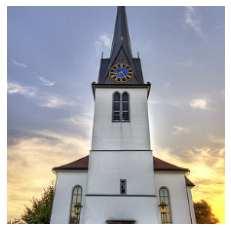
\includegraphics[width=.32\columnwidth]{Figures/related/attacks/bim_1_chicken.png}
                &
        
\includegraphics[width=.32\columnwidth]{Figures/related/attacks/bim_1_chicken_diff2.png}
        \\
        (B) BIM & (C) $(B - A)$ \\
        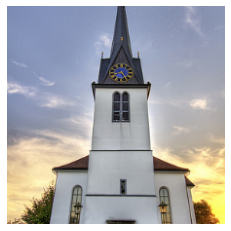
\includegraphics[width=.32\columnwidth]{Figures/related/attacks/ddn_0.85_chicken.png}
                &
        
\includegraphics[width=.32\columnwidth]{Figures/related/attacks/ddn_0.85_chicken_diff2.png}
        \\
        (D) DDN & (E) $(D - A)$ \\
        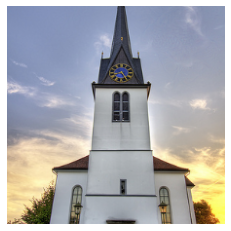
\includegraphics[width=.32\columnwidth]{Figures/related/attacks/cw_0.62_chicken.png}
                &
        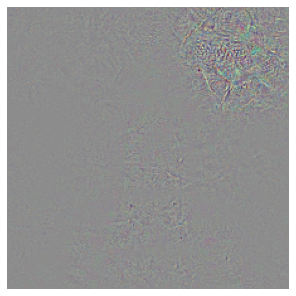
\includegraphics[width=.32\columnwidth]{Figures/related/attacks/cw_0.62_chicken_diff2.png}
        \\
        (F) CW  & (G) $(F - A)$
    \end{tabular}
    \caption{ Adversarial examples generated with different methods. The
        original input image (A) is correctly classified as a "church", while
        all the generated samples: (B), (D) and (F) are identified as a
        "chicken" by the model. }
    \label{fig:samples_ae}
\end{figure}

\clearpage


%---------------------------------------------------------------------
\section{Defending Against Adversarial Examples}
\label{sec:defending_adgainst_adversarial_examples}

Since Christian Szegedy \emph{et al} \cite{szegedy_intriguing_2014} discovered
the existence of adversarial examples, much research has been conducted from the
perspectives of both the attacker, \emph{i.e.,} the party trying to exploit
vulnerabilities in a model and the defending party trying to mitigate these
attacks. The authors also hypothesized that adversarial examples exist due to
the high non-linearity nature of NNs. However, this hypothesis was later
rebutted by Goodfellow \emph{et al} when they argued that adversarial examples
exist due to NNs being too linear rather than the contrary
\cite{goodfellow_explaining_2015}.

The research first focused on defending against adversarial examples by
improving the robustness of neural networks via, among others, adversarial
training \cite{goodfellow_explaining_2015,papernot_limitations_2015}, where
adversarial examples are included in a dataset alongside natural images in order
to train a CNN on both natural images and adversarial samples. The computational
cost required to generate adversarial examples makes this defense approach
computationally expensive, even when using techniques such as FGSM that require
\emph{considerably} less computational work than methods such as CW which can
require hours to generate a single sample on a low-end gpu.

\textit{Defensive distillation} \cite{papernot_distillation_2016} is another
technique to improve the robustness of NN and involves the use of two networks.
A first network $F$ is conventionally trained on inputs $X$ and labels $Y$ and
outputs a probability vector predictions $F(X)$. The second network $F_{d}$ is
then trained on the same inputs $X$, but the labels are replaced by the output
of the first network $F(X)$ as a way of restraining the model from over-fitting
on the data. Defensive distillation is a very effective defense but was defeated
by the more recent CW attack.

Due to the difficulty and computational cost of training robust neural networks
against adversarial examples, recent research has focused on detecting them
instead. However, a recent survey by N. Carlini and D. Wagner examined ten
detection defenses that they all bypassed using their attack method and
concluded that adversarial examples are significantly more complex to detect
than previously recognized \cite{carlini_adversarial_2017}. Furthermore, among
the ten detection methods surveyed, they concluded that only \textit{bayesian
neural network uncertainty} \cite{feinman_detecting_2017} was effective and made
generating adversarial examples nearly five times more difficult on the dataset
CIFAR-10. For their method, Reuben Feinman \emph{et al} use dropout
\cite{srivastava_dropout_2014} to induce randomness during inference and predict
an input multiple times in order to measure the prediction uncertainty. They
show that the prediction uncertainty is typically higher on adversarial examples
compared to normal and noisy images.

\section{Detection Evaluation Metrics}
To attest to the effectiveness of the detection performances of the method
proposed in a later section, I adopt the recall and precision rates defined as
\begin{align} \label{eq:recall}
    recall=\frac{tp}{tp+fn},
\end{align}
where $tp$ (\textit{true positive}) is the number of correctly detected
adversarial examples and $fn$ (\textit{false negative}) is the number of
adversarial examples that are not detected.
\begin{align} \label{eq:precision}
    precision=\frac{tp}{tp+fp},
\end{align}
where $fp$ (\textit{false positive}) is the number of normal images that are
incorrectly identified as adversarial examples.

Finally, we use the $F_{\beta}$ score defined as:
\begin{align} \label{eq:fb}
    F_{\beta}=(1+\beta^{2})\frac{recall\cdot
        precision}{recall+(\beta^{2}precision)},
\end{align}
where $\beta=2$ to emphasize on the recall rate.


\chapter{Experiments}
\label{Experiments}
\overridetextsize

\section{Overview}
\label{sec:experiments_overview}


Adversarial examples can be seen as a worst-case noise that fools the model into
misclassification when applied to an image. On the other hand, neural networks
are relatively robust to random corruptions such as Gaussian noise.

My intuition is that applying random noise to an adversarial example could hide
or alter parts of the adversarial perturbation, thus diminishing or even
nullifying its effect.

In order to apply a random transformation to an image $x$, we generate a
Gaussian noise $\tilde{y}=\mathcal{N}(0,1)$ that we add to the image in order to
create a noisy version $\tilde{x}$:
\begin{align} \label{eq:noisy_version}
    \tilde{x}=x+\tilde{y}\kappa,
\end{align}
where $\kappa$, is the standard deviation used to scale down or up the noise
intensity.

\begin{figure}
    \subfloat[]{%
        \includegraphics[clip,width=.33\linewidth]{Figures/noise/std:0.0,l2:
            0.0,PSNR:100.0.png}%
    } \subfloat[]{%
        \includegraphics[clip,width=.33\linewidth]{Figures/noise/std:0.02,l2:
            5.1,PSNR:34.01.png}%
    } \subfloat[]{%
        \includegraphics[clip,width=.33\linewidth]{Figures/noise/std:0.04,l2:
            10.13,PSNR:28.05.png}%
    }

    \subfloat[]{%
        \includegraphics[clip,width=.33\linewidth]{Figures/noise/std:0.06,l2:
            15.07,PSNR:24.6.png}%
    } \subfloat[]{%
        \includegraphics[clip,width=.33\linewidth]{Figures/noise/std:0.08,l2:
            19.91,PSNR:22.18.png}%
    } \subfloat[]{%
        \includegraphics[clip,width=.33\linewidth]{Figures/noise/std:0.1,l2:
            24.61,PSNR:20.34.png}%
    }

    \caption{ Increasing the noise intensity $k$ on an ImageNet sample. Details
        in Table \ref{table:noise_increase}.}
    \label{fig:noise_increase}
\end{figure}

Fig \ref{fig:noise_increase} shows the impact of increasing $\kappa$ on an image
and shows the corresponding $L_2$ distance and peak signal-to-noise ratio (PSNR)
of the noise mask.

\begin{table}[htb]
    \centering
    \begin{tabular}{c c c c}
        \toprule
        Image & $k$  & $L_{2}$ & PSNR  \\
        \midrule
        A     & 0.00 & 0.00    & 100   \\
        B     & 0.02 & 7.76    & 34.01 \\
        C     & 0.04 & 15.46   & 28.05 \\
        D     & 0.06 & 23.11   & 24.60 \\
        E     & 0.08 & 30.40   & 22.18 \\
        F     & 0.10 & 37.36   & 20.34 \\
        \bottomrule
    \end{tabular}
    \caption{Details for Figure \ref{fig:noise_increase}}
    \label{table:noise_increase}
\end{table}

To further motivate and formulate the proposed method discussed in section
\ref{Methodology}, I first perform a series of experiments detailed in the
remainder of this section to verify that the intuition mentioned above holds
correct.

\section{Experimental Settings}
Below I describe the datasets and models used, as well as the settings used to
configure the attack methods.

\subsection{Datasets and Models}
\label{sub:datasets_models}

To conduct the experiments, I collect data from three datasets:
\begin{itemize}
    \item CIFAR-10 \cite{krizhevsky_learning_2009}, widely used dataset
          consisting of 60000 $32 \times 32$ RGB images divided into ten
          different classes (e.g., airplane, automobile, bird.). For the
          experiments, I use the 10.000 images present in the test set.
    \item ImageNet \cite{russakovsky_imagenet_2015}, popular image database
          containing over 1.300.000 $224 \times 224$ RGB images divided into
          1000 different classes. For our experiments, rather than using the
          entirety of the dataset, I created a subset containing 10 of ImageNet
          classes.
    \item Dogs vs. Cats \cite{elson_asirra_2007}, the Asirra (Animal Species
          Image Recognition for Restricting Access) is a real-world Kaggle
          dataset containing 25.000 $224 \times 224$ resized RGB images divided
          into two classes: dogs and cats.
\end{itemize}

For the models, we use a Very Deep Convolutional Networks for Large-Scale Image
Recognition with 11 layers \cite{simonyan_very_2015-2}. The
complete architecture of the VGG-11 model is shown in table \ref{table:vgg11}.

\begin{table}[htb]
    \centering
    \begin{tabular}{c c}
        \toprule
           & VGG 11             \\
           & Input (224x224x3)  \\
        \midrule
        1  & Conv. 64           \\
           & Maxpool            \\
        \hline
        2  & Conv. 128          \\
           & Maxpool            \\
        \hline
        3  & Conv. 256          \\
        4  & Conv. 256          \\
           & Maxpool            \\
        \hline
        5  & Conv. 512          \\
        6  & Conv. 512          \\
           & Maxpool            \\
        \hline
        7  & Conv. 512          \\
        8  & Conv. 512          \\
           & Maxpool            \\
        \hline
        9  & FC 4096            \\
        10 & FC 4096            \\
        11 & FC 1000 ($\sigma$) \\
        \bottomrule
    \end{tabular}
    \caption{VGG configuration with 11 layers}
    \label{table:vgg11}
\end{table}

We use pre-trained on ImageNet models open-sourced by PyTorch for the
experiments using the ImageNet and Dogs vs. Cats datasets. For Dogs vs. Cats,
the model is fined-tuned, \emph{i.e.,} the last few layers' parameters are
updated instead of training the whole network from scratch.

\subsection{Attacks}
\label{sec:attack}
I implement the attacking methods introduced in Section
\ref{Adversarial_examples} using the FoolBox library \cite{rauber_foolbox_2020}.
For targeted attacks defined in section \ref{Adversarial_examples}, the target
$t$ class is selected randomly such that
\begin{align} \label{eq:targeted}
    \left\{ t:t\in C \backslash \left\{
    y\right\}\right\},
\end{align}
where $C$ is a set of the available classes in the dataset and $y$ is the
ground-truth label of the sample.

I generate adversarial examples using accurately classified images from the test
sets of each dataset as it would not make sense generating adversarial examples
on samples that the models already fail to identify.

\section{Robustness}
\label{sec:robustness}

In this section, in order to verify the intuition mentioned in section
\ref{sec:experiments_overview}, I describe two experiments where I apply noise
to both the input images and the adversarial examples in order to compare the
model's output before and after the added noise.


\subsection{Consistency}
\label{sub:consistency}

\begin{figure}[htp]
    \subfloat[]{%
        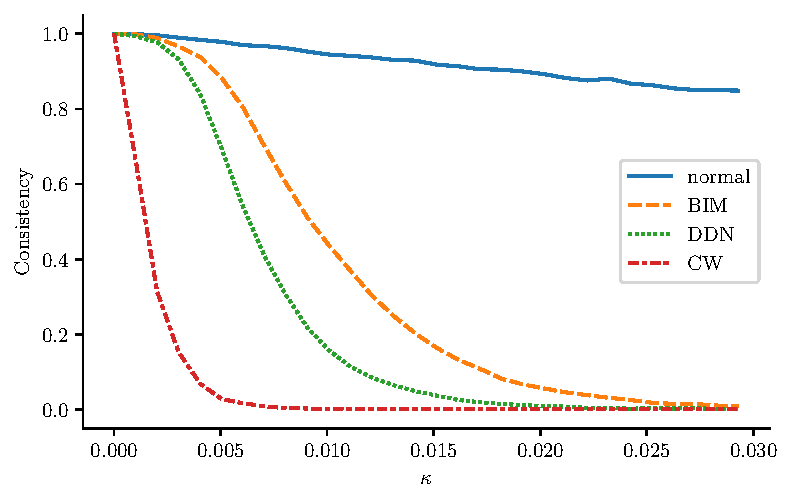
\includegraphics[clip,width=\columnwidth]{figures/fig2a.pdf}%
    }

    \subfloat[]{%
        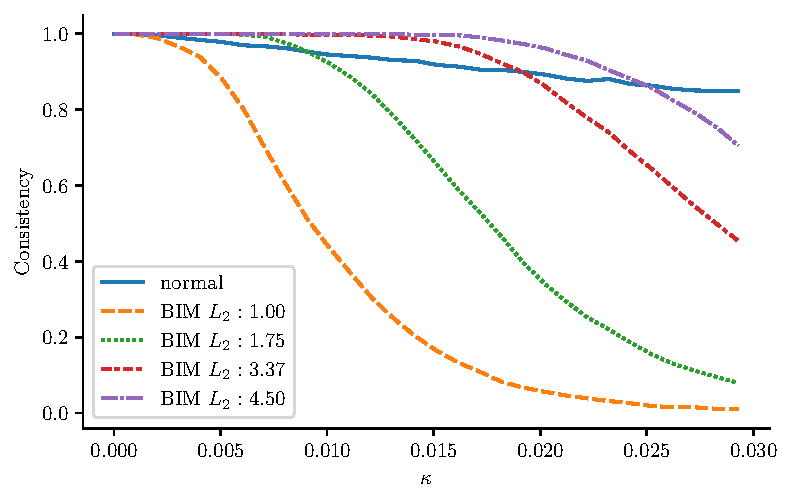
\includegraphics[clip,width=\columnwidth]{figures/fig2b.pdf}%
    }

    \caption{Consistency comparison between normal images and adversarial
        examples using different methods and perturbation budgets. As $\kappa$
        (see \eqref{eq:noisy_version}) increases, the consistency decreases,
        more so for adversarial examples, unless we also increase the
        adversarial perturbation budget as seen in (b).}
    \label{fig:consistency}
\end{figure}


In the first experiment, I compare the model's classification output for a
normal image $x$ and a transformed version $\tilde{x}$ (Eq.
\eqref{eq:noisy_version}). When the classifications $C(x)$ and $C(\tilde{x})$
are identical, I refer to them as being \emph{consistent} classifications.
\emph{i.e.,} when the model predicts the same class for the unperturbed image
and the same image but containing voluntarily added noise, the predictions are
consistent with one other. If my intuition is correct, we should observe the
predictions on normal images to be more consistent when adding noise. At the
same time, I expect the model's predictions on adversarial examples to start
being more inconsistent as the noise intensity increases.

Here, our objective is to compare the consistency between normal images and
adversarial examples. To proceed, I randomly select 1000 images from ImageNet's
test set to record the classification consistency on each sample and at
different $\kappa$ (Eq. \eqref{eq:noisy_version}) values. Finally, we follow the
same procedure for adversarial examples and generate 1000 samples with the BIM,
DDN, and CW methods.

Figure \ref{fig:consistency} shows the average classification consistency of
input types and at different $\kappa$. We observe the average consistency to
decrease slowly as $\kappa$ increases for normal images. This moderate decrease
shows that, as expected, the model is not significantly affected by the random
perturbation added to the image. On the contrary, we observe that adversarial
examples' classification consistency decreases rapidly as $\kappa$ increases.
These results corroborate my intuition that introducing random perturbations to
an adversarial example could impede its effectiveness.

\begin{figure}[ht]
    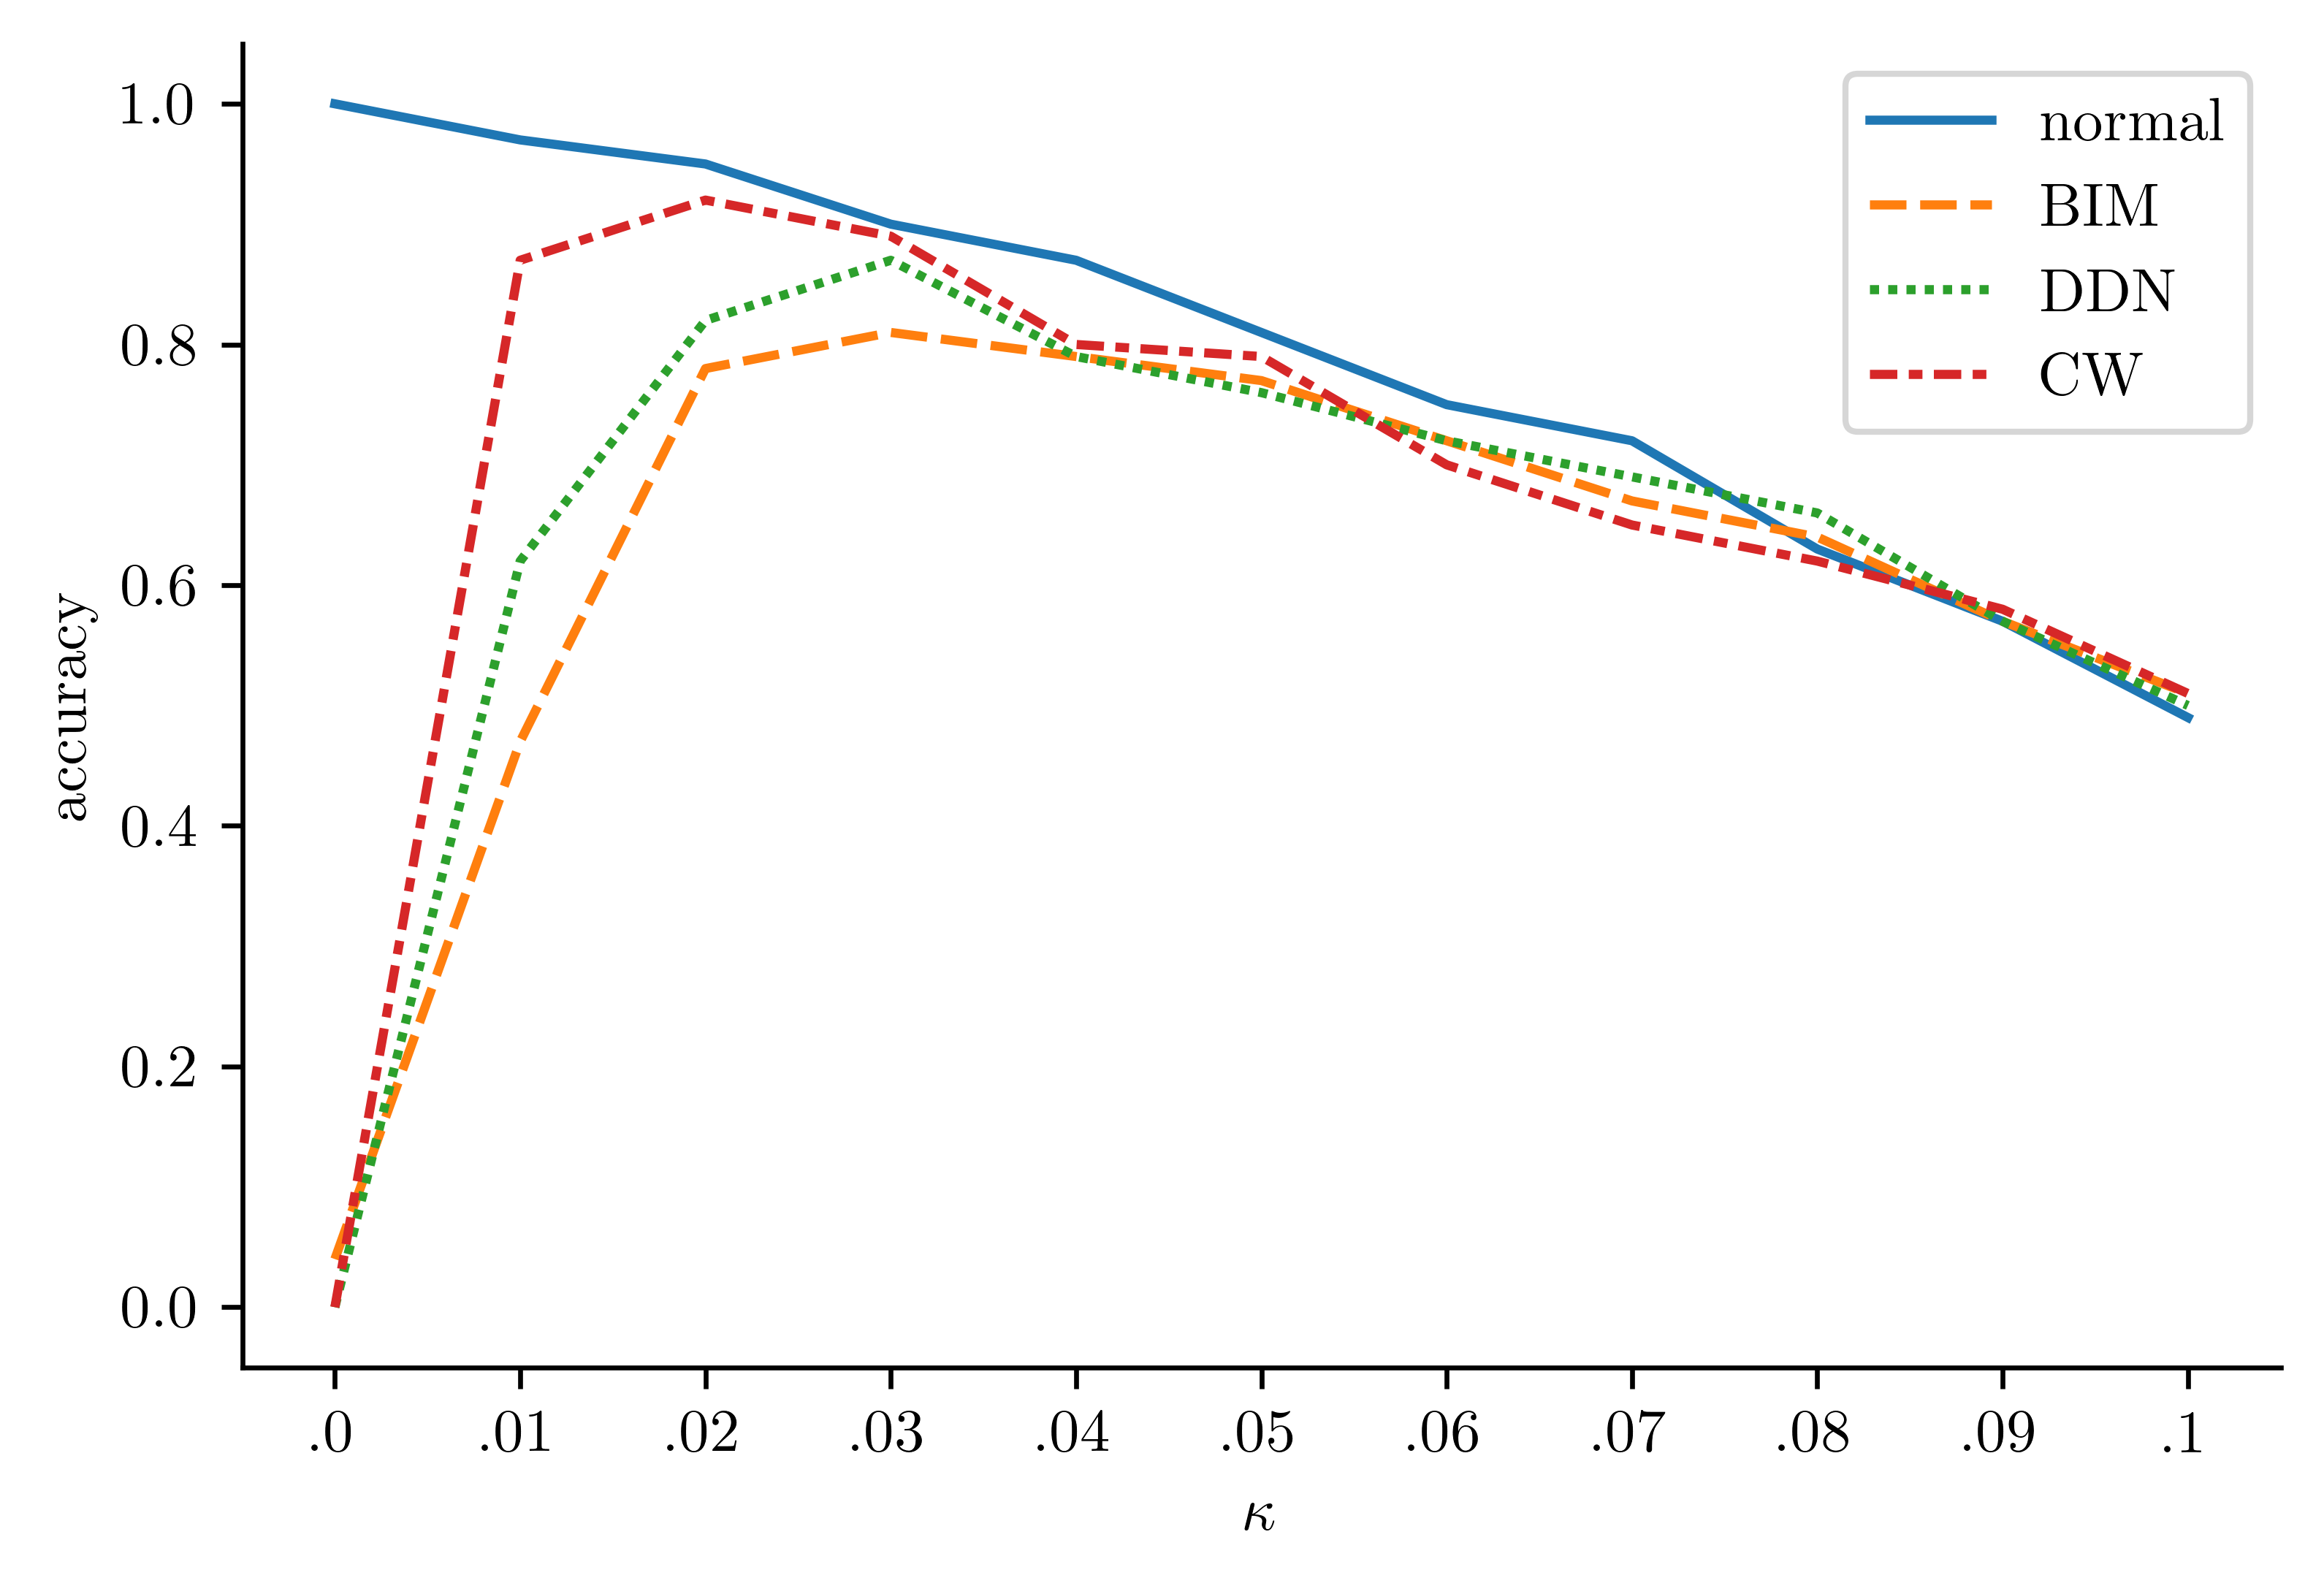
\includegraphics[width=\columnwidth]{Figures/experiments/accuracy.png}%
    \caption{Shows the accuracy comparison between normal images and adversarial
        examples; as $\kappa$ increases, the accuracy of adversarial examples first
        increases before decreasing similarly to normal images.}
    \label{fig:accuracies}
\end{figure}

Furthermore, figure \ref{fig:accuracies} shows that the actual prediction
accuracies are partially restored on adversarial examples as the noise intensity
increases before slowly reducing again, similarly to normal images, when the
noise intensity is too high for the model. Finally, average accuracies of normal
images and adversarial examples start to be very similar at around $0.03
    \kappa$, hinting and showing again that the adversarial perturbations in
adversarial examples lost their efficacy to fool the targeted models.


Interestingly, coming back to figure \ref{fig:consistency}A, we can also observe
the classification consistency being different between attacking methods,
\emph{i.e.,} to reach a consistency of $\approx 0$, adversarial examples
generated with BIM need a larger $\kappa$ than samples generated with DDN and
CW.

Instinctively, this difference makes sense; adversarial examples generated with
the BIM approach have a larger average $L_2$ adversarial perturbation of
$\approx 1.0$ compared with DDN at $L_2\approx0.85$ and CW at $L_2\approx0.70$.
Figure \ref{fig:consistency}b shows the same experiment but using adversarial
examples generated with BIM at different perturbation budgets. These results
undeniably show that the more substantial the adversarial perturbation is
(\emph{i.e.,} higher perturbation budget), the more robust it is to random
perturbations. Therefore, a larger $\kappa$ may be needed to counter the
effectiveness of the higher adversarial perturbation budget attacks.

\subsection{Logits differences}
\label{sub:logits_differences}
\begin{figure}[ht]
    \centering
    \subfloat[Normal Image]{%
        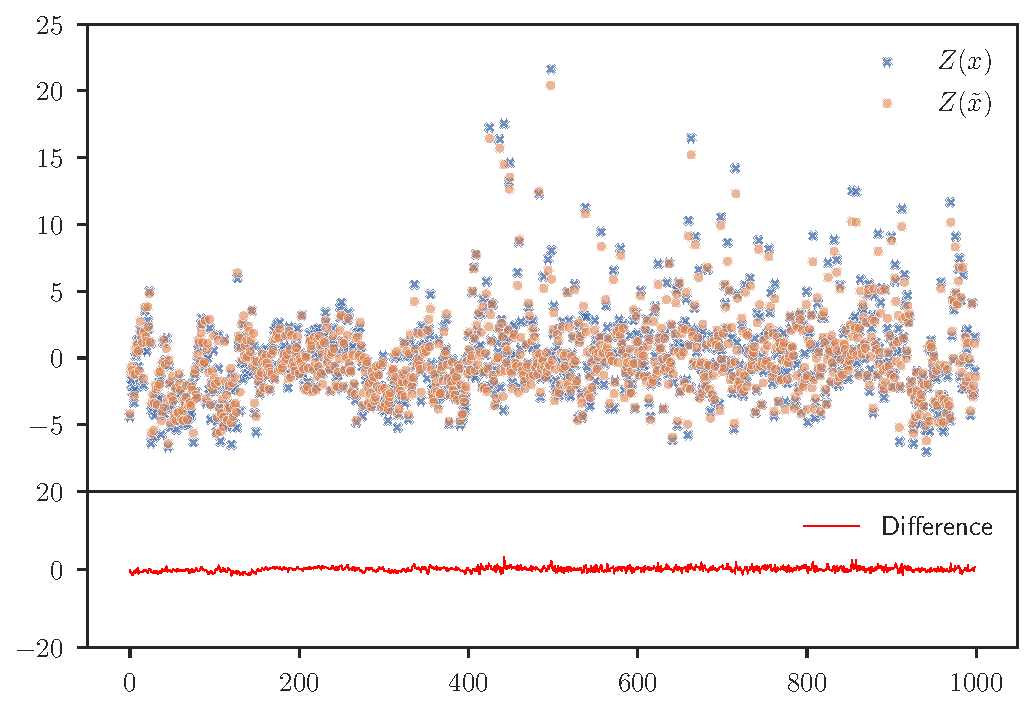
\includegraphics[clip,width=0.9\columnwidth]{figures/fig4a.pdf}%
    }

    \subfloat[Adversarial Example (BIM)]{%
        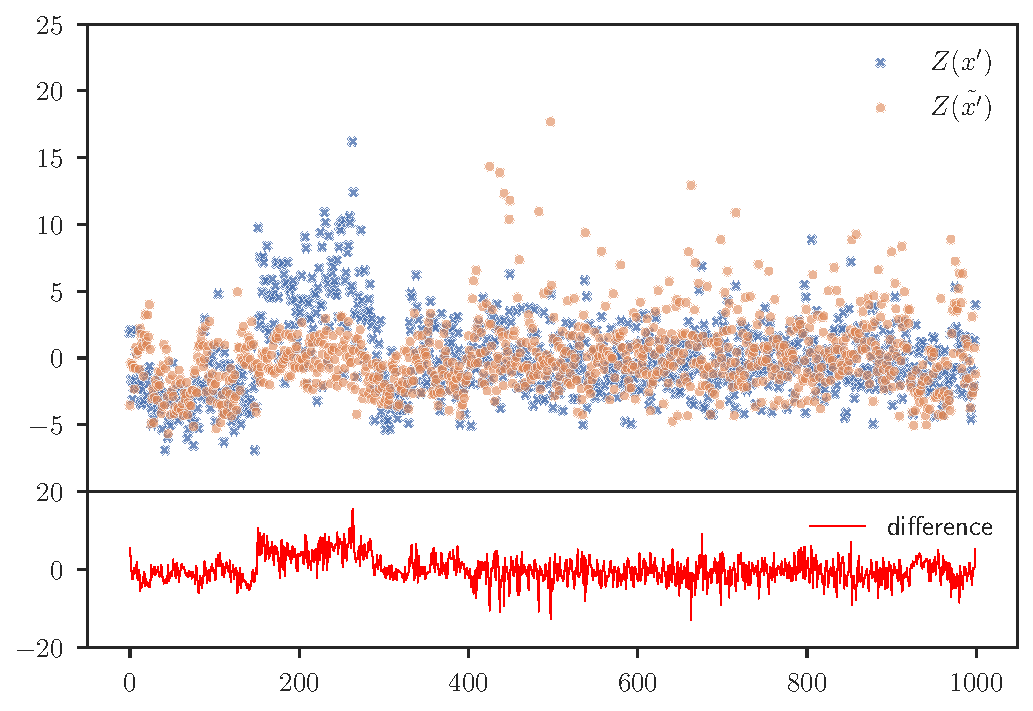
\includegraphics[clip,width=0.9\columnwidth]{figures/fig4b.pdf}%
    } \caption{Comparison between the logits of an ImageNet image before
        ($Z(x)$) and after adding noise to the input ($Z(\tilde{x})$). When the
        input is normal (A), the difference between predictions is small, but
        becomes larger when the input is adversarial (B).}
    \label{fig:logits}
\end{figure}

I performed another experiment to investigate further the difference between the
model output for an untransformed and a randomly perturbed image. Instead of
recording the classification output of the model as done in section
\ref{sub:consistency}, which is only a reduced-down portion of the output, I
decided to observe the output logits, \emph{i.e.,} the output before applying
the activation function: in this case, before applying softmax. This will allow
us to see the raw output values for each class.

I select a single ImageNet image $x$ and generate a noisy version $\tilde{x}$
with $\kappa=\num{2e-2}$. Figure \ref{fig:logits}A shows the output logits
$Z(x)$ and $Z(\tilde{x})$ for each the normal image $x$ and the perturbed
version $\tilde{x}$ respectively. Logits are plotted (1000 logits for the 1000
ImageNet classes), as well as the difference between $Z(x)_i$ and
$Z(\tilde{x})_i$ in the lower part of the plot. We observe both outputs to be
very similar value-wise for each class. On the contrary, when the original input
is adversarial (BIM, $L_2 \approx 1$), as in figure \ref{fig:logits}B, the
difference between outputs is striking, magnitudes over the difference observed
with the normal image.

These two experiments proved that my initial intuition was correct. It also
showed that the higher budget the adversarial perturbation, the more robust it
is against the random perturbation I add to the input. To me, this may explain
why many detection techniques fail to detect higher-perturbation budgets
adversarial examples. These observations motivated me to pursue this track
because I believe that the ease with which we can add varying random
perturbation to the input, by increasing or decreasing $\kappa$, could be an
interesting idea to combat low \emph{and} high perturbation budgets attacks.

Observing and comparing the model outputs showed us that adding a random
perturbation to an image can help us detect the legitimate or adversarial nature
of the input.

Following these observations, I present in the following section a novel method
to detect adversarial examples.


\chapter{Proposed Methodology}
\label{Methodology}
\overridetextsize

\section{Noise-Aided Adversarial Example Detection (NAED) Method}
As observed during the experiments conducted in section \ref{sub:consistency}
and section \ref{sub:logits_differences}, the usage of Gaussian noise to alter
the efficacy of the perturbations present in adversarial examples is effective.
To build upon these observations, I propose a methodology to detect adversarial
examples that I describe in the remainder of this section.

This methodology, represented in figure \ref{fig:framework}, aims to compute two
scores, described in the following subsection, using the difference in
predictions before and after applying random noise to the input image space.
From the two scores computed for each input, we can determine if an input is
adversarial or not.

\begin{figure}[htp]
    \centering
    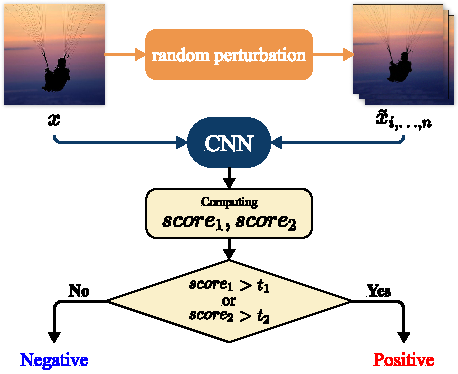
\includegraphics[clip,width=0.9\columnwidth]{Figures/methodology/Framework.pdf}%

    \caption{The framework of the discussed method.}
    \label{fig:framework}
\end{figure}

\section{Predictions Differences: Two scores}
\label{sub:detection_metrics}
As observed in section \ref{sub:logits_differences}, the model predictions
differ to a more significant degree when adversarial examples are perturbed by
additive random noise compared with normal images.

To capture these differences, we use two scores defined as follows:
\begin{align}
    \label{eq:score1}
    score_{1}{(x,\tilde{x})}=\sqrt{\frac{1}{N}\sum_{i=1}^{N}(d_{i}-\mu)^{2}},
\end{align}
where $d$ is the element-wise difference between two sets of logits:
\begin{align}
    \label{eq:diff}
    d=(Z(x)-Z(\tilde{x})),
\end{align}
and $\mu$ is the mean:
\begin{align}
    \label{eq:mean_mu}
    \mu=\frac{1}{N}\sum_{i=1}^{N}d_{i}.
\end{align}

Thus, $score_{1}$ computes the element-wise difference between two sets of
logits and calculate the standard deviation of the remaining vector.

The second score similarly compares two sets of predictions by computing the
$L_1$-norm, or Manhattan distance, as follows:
\begin{align}
    \label{eq:score2}
    score_{2}{(x,\tilde{x})}=||F(x)-F(\tilde{x})||_{1}.
\end{align}

Notably, $score_{1}$ uses the model's raw output, \emph{i.e.,} logits, whereas
$score_{2}$ uses the output of the softmax layer.

\begin{figure}[htp]
    \subfloat[Normal images compared with different adversarial examples
        generation methods.]{%
        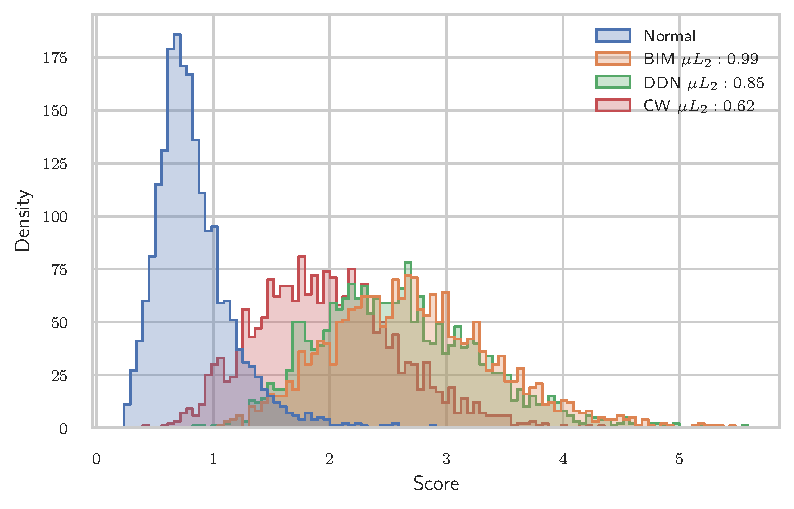
\includegraphics[clip,width=\columnwidth]{Figures/methodology/Fig5a.pdf}%
    }

    \subfloat[Normal images compared with BIM-generated samples at varying
        perturbation budgets.]{%
        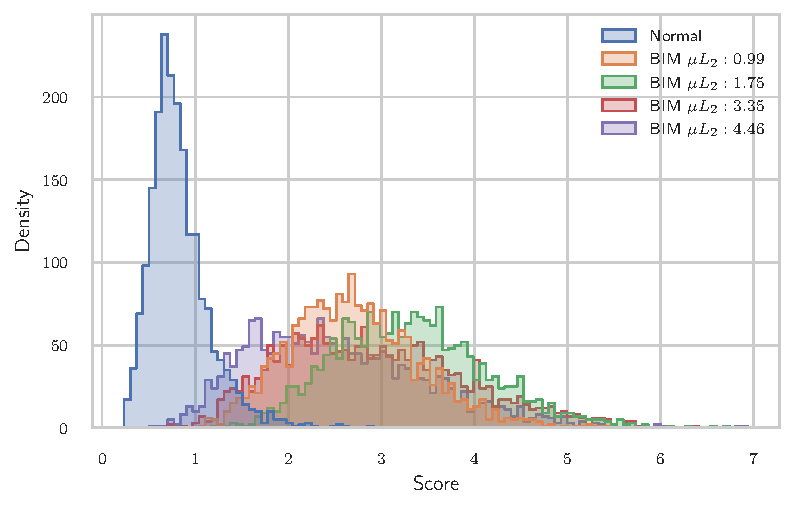
\includegraphics[clip,width=\columnwidth]{Figures/methodology/Fig5b.pdf}%
    }

    \caption{Histograms showing the $score_{1}$ per sample type.}
    \label{fig:score_1}
\end{figure}


\begin{figure}[htp]
    \subfloat[Normal images compared with different adversarial examples
        generation methods.]{%
        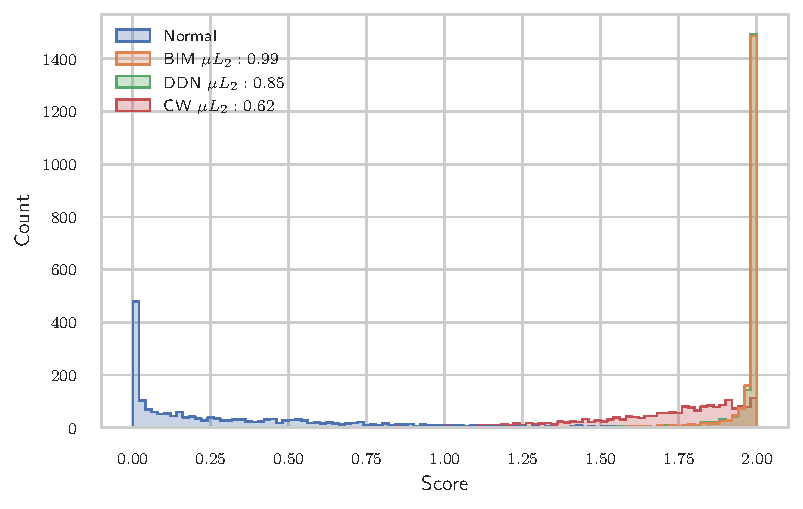
\includegraphics[clip,width=\columnwidth]{Figures/methodology/Fig6a.pdf}%
    }

    \subfloat[Normal images compared with BIM-generated samples at varying
        perturbation budgets.]{%
        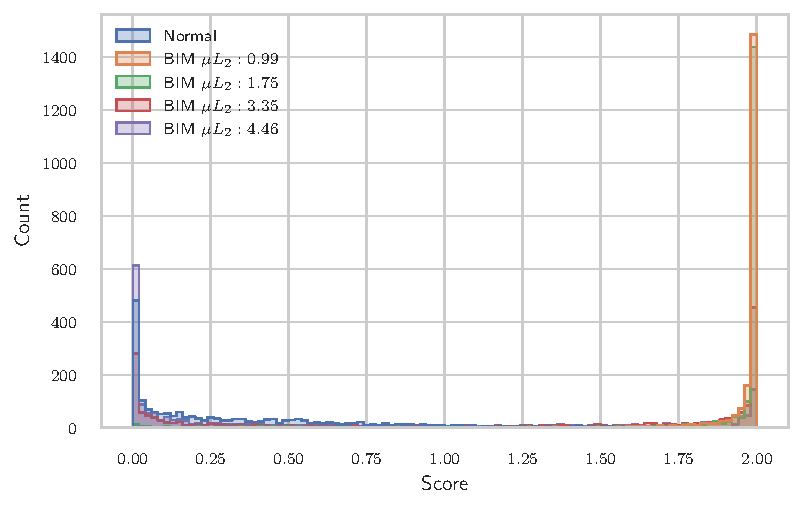
\includegraphics[clip,width=\columnwidth]{Figures/methodology/Fig6b.pdf}%
    }

    \caption{Histograms showing the $score_{2}$ per sample type.}
    \label{fig:score_2}
\end{figure}

As seen in figures \ref{fig:score_1} and \ref{fig:score_2}, using a $\kappa$ of
$0.03$, we observe the distribution of normal images and adversarial examples
differs. However, we can observe in \ref{fig:score_2}B that when the
perturbation budget increases, the distribution of adversarial samples starts to
join the same distribution as normal images. Each score performs differently for
various attacking methods and perturbation budgets. Notably, $score_{1}$ seem to
be less affected by the perturbation budgets of the attacks, offering a better
generalization.

\newpage

\section{Threshold-based Detection: A Method-Specific Approach}
\label{sec:method_specific_approach}
\begin{figure}[htp]
    \subfloat[$score_1$ ImageNet]{%
        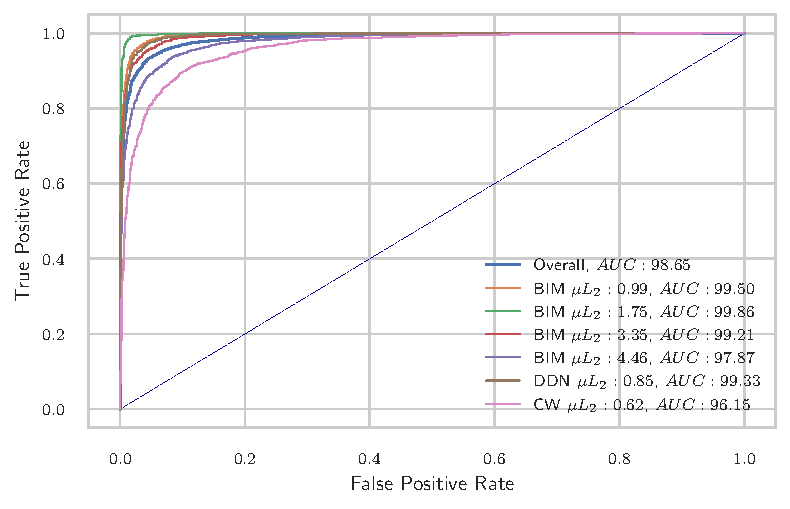
\includegraphics[clip,width=.5\columnwidth]{Figures/methodology/Fig7a.pdf}%
    }
    \subfloat[$score_2$ ImageNet]{%
        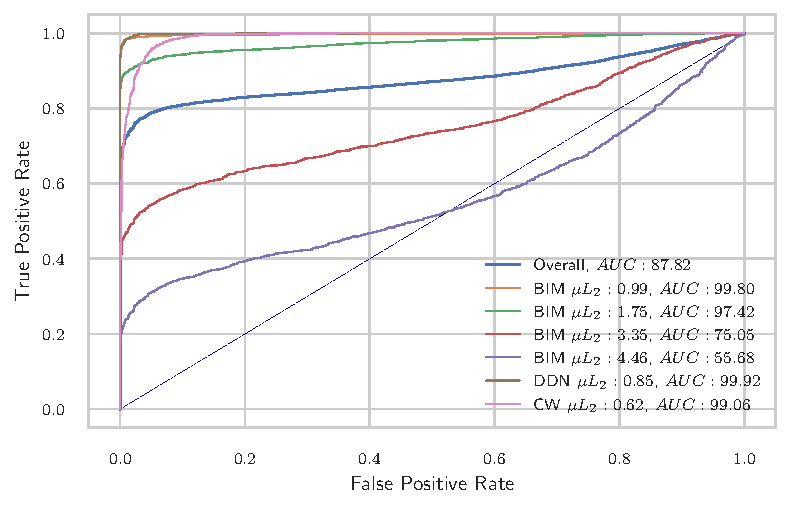
\includegraphics[clip,width=.5\columnwidth]{Figures/methodology/Fig7d.pdf}%
    }

    \subfloat[$score_1$ D. vs. C.]{%
        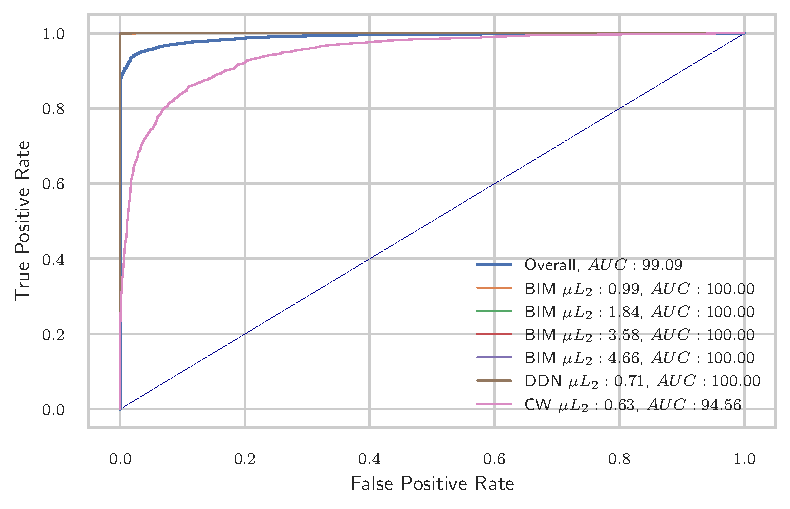
\includegraphics[clip,width=.5\columnwidth]{Figures/methodology/Fig7b.pdf}%
    } \subfloat[$score_2$ D. vs. C.]{%
        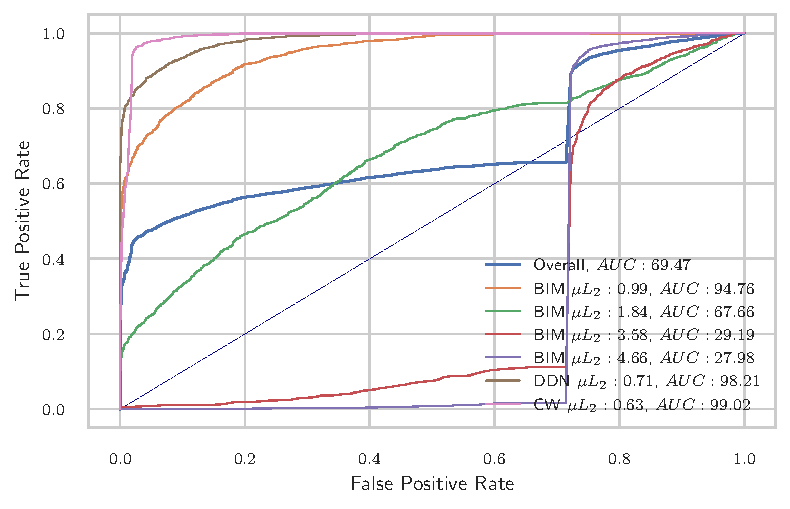
\includegraphics[clip,width=.5\columnwidth]{Figures/methodology/Fig7e.pdf}%
    }

    \subfloat[$score_1$ CIFAR-10]{%
        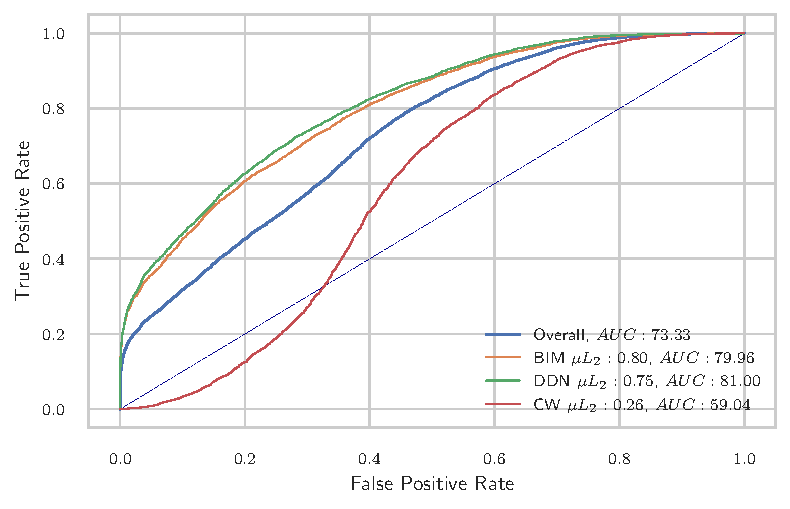
\includegraphics[clip,width=.5\columnwidth]{Figures/methodology/Fig7c.pdf}%
    }
    \subfloat[$score_2$ CIFAR-10]{%
        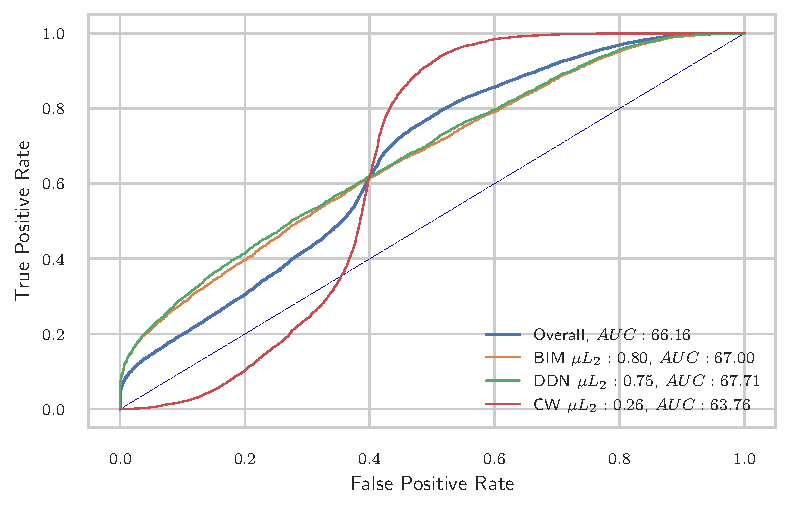
\includegraphics[clip,width=.5\columnwidth]{Figures/methodology/Fig7f.pdf}%
    }
    \caption{ROC-AUC for each classifier and each dataset.}
    \label{fig:rocs}
\end{figure}

To demonstrate the effectiveness of each metric in a detection scenario, we
build a threshold-based binary classifier for each attacking method on each
dataset. The classifiers can either classify an input as negative (normal
images) or positive (adversarial example). Figure \ref{fig:rocs} shows the
Receiver Operating Characteristic Curve (ROC) and Area Under the Curve (AUC) of
each classifier. Following my previous observations, we verify again that
$score_1$ can effectively identify adversarial examples from diverse methods and
even at different perturbation sizes, showing an overall AUC of 98.65\% on
ImageNet and 99.09\% on Dogs vs. Cats.

\section{Adapting to Production: Method-Agnostic Approach}
This method-specific approach described previously is suitable for displaying
each classifier's best available result. Unfortunately, it is not a realistic
scenario in a production environment as we would not be aware of the exact
nature of the input. Furthermore, it would require training a classifier for
each attack method at different perturbation sizes.

I propose an approach to select a threshold for the metric scores, only relying
on the normal images present in the initial datasets to solve this problem. This
approach offers great flexibility and adaptability as we do not require prior
knowledge of the attacking method used to generate an adversarial sample. It is
essential to select a suitable threshold as the detection effectiveness depends
ultimately on it; if the threshold is too high, the number of false positives
will be high and vice versa for false negatives.

\subsection{Threshold and Noise Intensity Selection}
\label{sec:selection_of_the_intensity}

Because of the relation between adversarial and random perturbation discussed in
Section \ref{sub:consistency}, to identify adversarial samples with diverse
adversarial budgets, we also need to generate random perturbations with a wide
range of intensity. To do so, I arbitrarily create a linearly spaced vector
containing ten $\kappa$ from \num{1e-2} to \num{1e-1} and accordingly generate
ten noisy images per given input. For each input pair $x$ and
$\{\tilde{x}\}_{i=1}^{10}$, I compute both $score_1$ (Eq. \ref{eq:score1}) and
$score_2$ (Eq. \ref{eq:score2}). The objective is to detect if a sample has an
abnormally large value with either of the scores.

To determine if a sample has an abnormally large value, we need to select a
threshold for each score \emph{i.e.,} at each noise intensity. To select these
thresholds, I first select 3000 training images from each dataset and record the
scores at each $\kappa$. The thresholds are then placed at the $99_{th}$ percentile
of these scores obtained on training images. Because the thresholds for each
score are determined solely using normal training images, my method does not
require prior knowledge of the attack to perform well.

I use BIM, DDN, and CW attack methods to validate this approach and generate 300
adversarial examples from images present in the ImageNet test set. I also select
100 normal images for the negative samples set.

Figure \ref{fig:distributions_scores} shows how many times each input was
positively detected. As expected, we can observe that most normal images are not
identified as positive once. In contrast, most adversarial examples are
identified as positive at least once. Note that, because we compute $score_1$
and $score_2$ at each ten selected $\kappa$, a sample can be identified from
zero to twenty times as positive.

\begin{figure}[p]
    \centering
    \subfloat[$score_1$]{%
        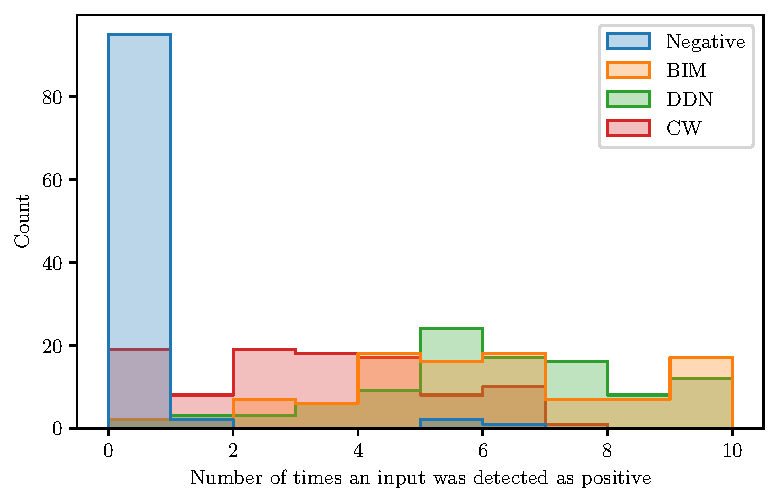
\includegraphics[clip,width=.7\textwidth]{Figures/methodology/distri_1.pdf}
    }

    \subfloat[$score_2$]{%
        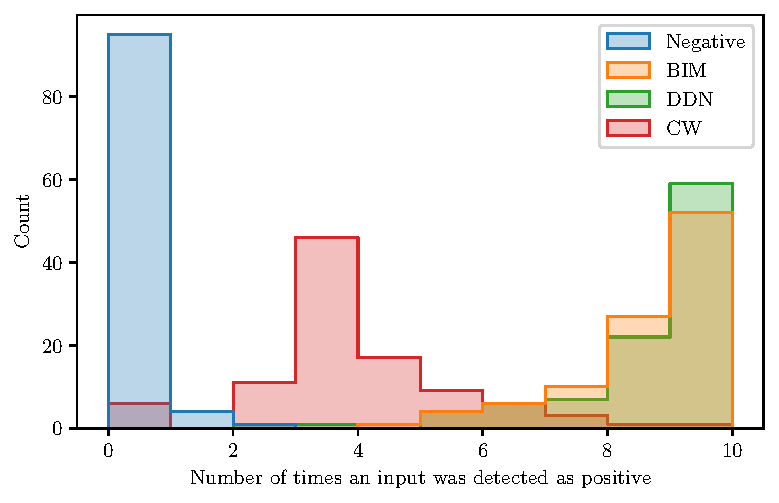
\includegraphics[clip,width=.7\textwidth]{Figures/methodology/distri_2.pdf}
    }

    \subfloat[Scores combined]{%
        \includegraphics[clip,width=.7\textwidth]{Figures/methodology/distri_combined.pdf}
    } \caption{Histograms showing the number of times an input was detected as
        positive on ImageNet.}
    \label{fig:distributions_scores}
\end{figure}

\newpage

\section{Detection Results and Performance Analysis}
\label{sec:detection_results}

Following the same procedure as in section \ref{sec:selection_of_the_intensity},
I evaluate the method with adversarial examples generated using different
approaches and various perturbation budgets. Table \ref{tab:detection_results}
shows the results of this evaluation. Using the combined scores, I observed a
high overall recall rate of 98.5\% on ImageNet and 100\% on Dogs vs. Cats. The
efficacy of each score depends on the type of attack used; for example,
$score_2$ does not perform as well on untargeted attacks but always performs
better on CW adversarial examples than $score_1$.

We also note that combining the scores shows to be a good strategy: for the cost
of a slight decrease in precision, the recall rate improves as well as the
overall $F_{\beta}$ score. With BIM, increasing the perturbation budget from an
average $L_2$ perturbation of $\approx 1.00$ to $\approx 3.00$ does not affect
the detection precision performances (Table \ref{tab:detection_results},
ImageNet/Dogs vs. Cats, No. 1- 3.).

Commonly, detection precision is higher when facing adversarial examples with
smaller perturbation sizes, such as samples generated with the CW attack method.
For instance, W. Xu \emph{et al} measure the $L_1$ distance between the
prediction vectors of the original image and its squeezed version
\cite{xu_feature_2018}, using bit depth reduction as well as local and non-local
spatial smoothing. As a result, they show comparable detection rates on
adversarial examples generated with the CW method, whereas the detection rate
falls to 55.56\% on samples crafted with BIM. However, using the same attack
settings (BIM$_\infty$, average $L_2$ of $\approx 1.40$), my approach
demonstrates a 100.0\% detection rate using the combined scores (Table
\ref{tab:detection_results}, ImageNet, No. 5). Therefore, a strength of my
method is that it can detect both low-perturbation and large-perturbation
adversarial examples.

This adaptability of our approach comes from the inputs being transformed with
varying random perturbation intensities, which allows for the detection of
samples generated with CW (at lower $\kappa$ values) and the detection of BIM or
similar methods (at higher $\kappa$ values). As seen in Table
\ref{tab:detection_results}, even when increasing the number of iterations from
100 (ImageNet, No. 7) to 10000 (ImageNet, No. 8) for samples generated with the
CW method, the detection performance remains unchanged. This is expected as
increasing the number of iterations does not make the perturbation more robust;
it only makes it less noticeable to the human eye.

\begin{table}[tph]
    \centering
    \begin{adjustbox}{angle=90}
        \resizebox{1.39\linewidth}{!}{%
            \begin{tabular}{c|c|cc|ccc|ccc|ccc|ccc}
                \toprule
                \multicolumn{1}{c}{\multirow{2}{*}{\rotcell{}}}         &
                \multirow{2}{*}{No.}                                    &
                \multirow{2}{*}{Attack}                                 &
                \multirow{2}{*}{$L_{2}$}                                & \multicolumn{3}{c|}{TP}        &
                \multicolumn{3}{c|}{Precision}                          & \multicolumn{3}{c|}{Recall}    &
                \multicolumn{3}{c}{$F_{\beta}$}                                                                           \\
                \multicolumn{1}{c}{}                                    &
                                                                        &                                &      &
                $score_1$
                                                                        &
                $score_2$
                                                                        &
                $combined$
                                                                        &
                $score_1$
                                                                        &
                $score_2$
                                                                        &
                $combined$
                                                                        &
                $score_1$
                                                                        &
                $score_2$
                                                                        &
                $combined$
                                                                        &
                $score_1$
                                                                        &
                $score_2$
                                                                        &
                $combined$
                \\
                \midrule
                \multirow{8}{*}{\begin{turn}{90}ImageNet\end{turn}}     & 1
                                                                        & \multirow{3}{*}{$BIM_{2}^{t}$} & 1.00 & 98
                                                                        &
                \textbf{100}
                                                                        &
                \textbf{100}
                                                                        & 0.951
                                                                        &
                \textbf{0.952}
                                                                        & 0.917
                                                                        & 0.980
                                                                        &
                \textbf{1.000}
                                                                        &
                \textbf{1.000}
                                                                        & 0.974
                                                                        &
                \textbf{0.990}
                                                                        & 0.982
                \\
                                                                        & 2
                                                                        &
                                                                        & 2.00                           &
                99
                                                                        &
                \textbf{100}
                                                                        &
                \textbf{100}
                                                                        &
                \textbf{0.952}
                                                                        &
                \textbf{0.952}
                                                                        & 0.917
                                                                        & 0.990                          &
                \textbf{1.000}
                                                                        &
                \textbf{1.000}
                                                                        & 0.982
                                                                        &
                \textbf{0.990}
                                                                        & 0.982
                \\
                                                                        & 3
                                                                        &
                                                                        & 3.00                           &
                95
                                                                        &
                \textbf{100}
                                                                        &
                \textbf{100}
                                                                        & 0.950
                                                                        &
                \textbf{0.952}
                                                                        & 0.917
                                                                        & 0.950                          &
                \textbf{1.000}
                                                                        &
                \textbf{1.000}
                                                                        & 0.950
                                                                        &
                \textbf{0.990}
                                                                        & 0.982
                \\
                                                                        & 4
                                                                        & $BIM_{2}$                      & 1.00
                                                                        & 96                             & 63
                                                                        &
                \textbf{98}
                                                                        &
                \textbf{0.950}
                                                                        & 0.926
                                                                        & 0.916                          &
                0.960                                                   & 0.630
                                                                        &
                \textbf{0.956}
                                                                        & 0.958
                                                                        & 0.673                          &
                \textbf{0.966}
                \\
                                                                        & 5
                                                                        & $BIM_{\infty}$                 & 1.40 & 99 & 70
                                                                        &
                \textbf{100}
                                                                        &
                \textbf{0.952}
                                                                        & 0.937
                                                                        & 0.917                          &
                0.990                                                   & 0.700
                                                                        &
                \textbf{1.000}
                                                                        &
                \textbf{0.982}
                                                                        & 0.737
                                                                        &
                \textbf{0.982}
                \\
                                                                        & 6
                                                                        & $DDN_{2}^{t}$                  & 0.85 & 98 &
                \textbf{100}
                                                                        &
                \textbf{100}
                                                                        & 0.951
                                                                        &
                \textbf{0.952}
                                                                        & 0.917
                                                                        & 0.980                          &
                \textbf{1.000}
                                                                        &
                \textbf{1.000}
                                                                        & 0.974
                                                                        &
                \textbf{0.990}
                                                                        & 0.982
                \\
                                                                        & 7
                                                                        & $CW_{2}^{t}$                   & 0.46 & 81 &
                \textbf{94}
                                                                        &
                \textbf{94}
                                                                        & 0.942
                                                                        &
                \textbf{0.949}
                                                                        & 0.913
                                                                        & 0.810                          &
                \textbf{0.940}
                                                                        &
                \textbf{0.940}
                                                                        & 0.833
                                                                        &
                \textbf{0.942}
                                                                        & 0.934
                \\
                                                                        & 8
                                                                        & $CW_{2}^{t}*$                  & 0.40 & 88 &
                \textbf{98}
                                                                        &
                \textbf{98}
                                                                        &
                \textbf{0.957}
                                                                        & 0.951
                                                                        & 0.925                          &
                0.880                                                   &
                \textbf{0.980}
                                                                        &
                \textbf{0.980}
                                                                        & 0.894
                                                                        &
                \textbf{0.974}
                                                                        & 0.968
                \\
                \midrule
                \multicolumn{4}{c|}{Total / Average}                    & 754
                                                                        & 725                            &
                \textbf{790}
                                                                        &
                \textbf{0.951}
                                                                        & 0.946
                                                                        & 0.918
                                                                        & 0.943
                                                                        & 0.906
                                                                        &
                \textbf{0.985}
                                                                        & 0.944
                                                                        & 0.911
                                                                        &
                \textbf{0.973}
                \\
                \midrule
                \multirow{5}{*}{\begin{turn}{90}Dogs vs Cats\end{turn}} & 1
                                                                        & \multirow{3}{*}{$BIM_{2}$}     & 1.00 &
                \textbf{100}
                                                                        & 72                             &
                \textbf{100}
                                                                        &
                \textbf{0.962}
                                                                        & 0.935
                                                                        & 0.926
                                                                        &
                \textbf{1.000}
                                                                        & 0.720
                                                                        &
                \textbf{1.000}
                                                                        &
                \textbf{0.992}
                                                                        & 0.755
                                                                        & 0.984
                \\
                                                                        & 2
                                                                        &
                                                                        & 2.00                           &
                \textbf{100}
                                                                        & 46
                                                                        &
                \textbf{100}
                                                                        &
                \textbf{0.962}
                                                                        & 0.902
                                                                        & 0.926                          &
                \textbf{1.000}
                                                                        & 0.460
                                                                        &
                \textbf{1.000}
                                                                        &
                \textbf{0.992}
                                                                        & 0.510
                                                                        & 0.984
                \\
                                                                        & 3
                                                                        &
                                                                        & 3.00                           &
                \textbf{100}
                                                                        & 41
                                                                        &
                \textbf{100}
                                                                        &
                \textbf{0.962}
                                                                        & 0.891
                                                                        & 0.926                          &
                \textbf{1.000}
                                                                        & 0.410
                                                                        &
                \textbf{1.000}
                                                                        &
                \textbf{0.992}
                                                                        & 0.460
                                                                        & 0.984
                \\
                                                                        & 4
                                                                        & $DDN_{2}$                      & 0.71
                                                                        &
                \textbf{100}
                                                                        & 88
                                                                        &
                \textbf{100}
                                                                        &
                \textbf{0.962}
                                                                        & 0.946
                                                                        & 0.926                          &
                \textbf{1.000}
                                                                        & 0.880
                                                                        &
                \textbf{1.000}
                                                                        &
                \textbf{0.992}
                                                                        & 0.892
                                                                        & 0.984
                \\
                                                                        & 5
                                                                        & CW$_{2}$                       & 0.53
                                                                        & 91                             & 99
                                                                        &
                \textbf{100}
                                                                        &
                \textbf{0.958}
                                                                        & 0.952
                                                                        & 0.926                          &
                0.910                                                   & 0.990
                                                                        &
                \textbf{1.000}
                                                                        & 0.919
                                                                        &
                \textbf{0.982}
                                                                        & 0.984
                \\
                \hline
                \multicolumn{4}{c|}{Total / Average}                    & 491
                                                                        & 346                            &
                \textbf{500}
                                                                        &
                \textbf{0.961}
                                                                        & 0.925
                                                                        & 0.926
                                                                        & 0.982
                                                                        & 0.692
                                                                        &
                \textbf{1.000}
                                                                        & 0.977
                                                                        & 0.720
                                                                        &
                \textbf{0.984}
                \\
                \midrule
                \multirow{6}{*}{\begin{turn}{90}CIFAR-10\end{turn}}     & 1
                                                                        & $BIM_{2}^{t}$                  & 0.75 &
                \textbf{67}
                                                                        & 46                             &
                \textbf{67}
                                                                        &
                \textbf{0.882}
                                                                        & 0.754
                                                                        & 0.798
                                                                        & 0.857
                                                                        & 0.460
                                                                        &
                \textbf{0.670}
                                                                        &
                \textbf{0.704}
                                                                        & 0.499
                                                                        & 0.692
                \\
                                                                        & 2
                                                                        & $BIM_{2}$                      & 0.75
                                                                        &
                \textbf{78}
                                                                        & 34
                                                                        &
                \textbf{78}
                                                                        &
                \textbf{0.897}
                                                                        & 0.694
                                                                        & 0.821                          &
                0.857                                                   & 0.340
                                                                        &
                \textbf{0.780}
                                                                        &
                \textbf{0.801}
                                                                        & 0.379
                                                                        & 0.788
                \\
                                                                        & 3
                                                                        & $BIM_{\infty}$                 & 1.00 &
                \textbf{85}
                                                                        & 40
                                                                        &
                \textbf{85}
                                                                        &
                \textbf{0.904}
                                                                        & 0.727
                                                                        & 0.833                          &
                0.857                                                   & 0.400
                                                                        &
                \textbf{0.850}
                                                                        &
                \textbf{0.860}
                                                                        & 0.440
                                                                        & 0.847
                \\
                                                                        & 4
                                                                        & $DDN_{2}$                      & 0.60
                                                                        & 78                             & 47
                                                                        &
                \textbf{79}
                                                                        &
                \textbf{0.897}
                                                                        & 0.758
                                                                        & 0.823                          &
                0.780                                                   & 0.470
                                                                        &
                \textbf{0.790}
                                                                        &
                \textbf{0.801}
                                                                        & 0.509
                                                                        & 0.796
                \\
                                                                        & 5
                                                                        & $CW_{2}$                       & 0.10
                                                                        & 28                             &
                \textbf{89}
                                                                        &
                \textbf{89}
                                                                        & 0.757
                                                                        &
                \textbf{0.856}
                                                                        & 0.840
                                                                        & 0.280                          &
                \textbf{0.890}
                                                                        &
                \textbf{0.890}
                                                                        & 0.320
                                                                        &
                \textbf{0.883}
                                                                        & 0.879
                \\
                                                                        & 6
                                                                        & $CW_{2}^{t}$                   & 0.22 & 37 &
                \textbf{82}
                                                                        &
                \textbf{82}
                                                                        & 0.804
                                                                        &
                \textbf{0.845}
                                                                        & 0.828
                                                                        & 0.370                          &
                \textbf{0.820}
                                                                        &
                \textbf{0.820}
                                                                        & 0.415
                                                                        &
                \textbf{0.825}
                                                                        & 0.822
                \\
                \midrule
                \multicolumn{4}{c|}{Total / Average}                    & 373
                                                                        & 338                            &
                \textbf{480}
                                                                        &
                \textbf{0.857}
                                                                        & 0.772
                                                                        & 0.824
                                                                        & 0.622
                                                                        & 0.563
                                                                        &
                \textbf{0.800}
                                                                        & 0.650
                                                                        & 0.589
                                                                        &
                \textbf{0.804}
                \\
                \bottomrule
            \end{tabular}
        }
    \end{adjustbox}
    \caption{Detection results for each dataset. Results are shown for both
        scores individually ($score_1$ and $score_2$) and combined ($combined$).
        For each attack, we specify the metric with which it was created
        ($\infty$ or $2$), whether the attack is targeted ($t$), and the
        corresponding average $L_2$ distance. \label{tab:detection_results}}
\end{table}

\pagebreak
\subsection{A Real-World Example: Showcasing the Method on a Sample}
To visualize a concrete example, I randomly select one image from the ImageNet
validation set where I perform the previously described method. I then generate
an adversarial example using BIM. Figure \ref{fig:showcase_example_samples}
shows the base image (A), the adversarial perturbation (B) magnified by ten, and
the final result adversarial example (C) that is identified as a "running shoe"
by the model.

\begin{figure}[htp]
    \subfloat[]{%
        \includegraphics[clip,width=.33\linewidth]{Figures/showcase_example/normal.png}%
    } \subfloat[]{%
        \includegraphics[clip,width=.33\linewidth]{Figures/showcase_example/ae_diff.png}%
    } \subfloat[]{%
        \includegraphics[clip,width=.33\linewidth]{Figures/showcase_example/ae.png}%
    }

    \caption{ Normal image (A), adversarial perturbation (magnified by 10) (B), adversarial example (C). }
    \label{fig:showcase_example_samples}
\end{figure}

\begin{figure}[htp]
    \subfloat[]{%
        \includegraphics[clip,width=.5\linewidth]{Figures/showcase_example/score_1_threshold.png}%
    } \subfloat[]{%
        \includegraphics[clip,width=.5\linewidth]{Figures/showcase_example/score_2_threshold.png}%
    }

    \caption{ comparing the number of times the thresholds are respected between
        a normal image and an adversarial example. $score_1$ in (A), $score_2$ in
        (B).  }
    \label{fig:showcase_scores}
\end{figure}

Processing \ref{fig:showcase_example_samples}A and
\ref{fig:showcase_example_samples}B through my approach gives us the results
shown in figure \ref{fig:showcase_scores}. Plot (A) shows us when a sample's
$score_1$ values exceed the threshold values. As expected and verified at the
beginning of this section, the normal image's scores values stay under the
corresponding thresholds. In contrast, the scores of the adversarial examples
exceed the thresholds in a few points; remember that exceeding the threshold at
any given noise intensity is enough to tag the image as being positive,
\emph{i.e.,} adversarial.

Similarly, with figure \ref{fig:showcase_scores}B, where we can
observe the same scenario happening, thresholds are exceeded by the adversarial
example while the normal image's scores remain under them.


\chapter{Discussion and Future Work}
\label{discussion}
\overridetextsize

\section{Addressing Low-Resolution Images}

One possible reason for the inferior detection performance on CIFAR-10 compared
to higher resolution datasets like ImageNet or Dogs vs. Cats, as shown in table
\ref{tab:detection_results}, is the relative size of the adversarial
perturbations required to fool the model. Lower-resolution images, such as those
in CIFAR-10, have fewer pixels and therefore require a more significant
proportion of pixels to be changed to create an adversarial example. This more
significant proportion of pixels changed can make the adversarial perturbations
more noticeable to the human eye. However, it also makes the perturbations more
robust to the random noise added to the image in the proposed method.
Additionally, the lower resolution of CIFAR-10 images may also impact the
ability of the model to classify the image accurately. This is because
lower-resolution images contain less visual information and may have less detail
than higher-resolution images. This lack of detail can make it harder for the
model to identify the important features for classification, which can make the
model more susceptible to adversarial examples. To improve the detection
performance on CIFAR-10, it may be necessary to use a more considerable value of
$\kappa$ to increase the amount of random noise added to the image. However,
increasing $\kappa$ too much can lead to the deterioration of normal images,
increasing false positives. Therefore, it is important to find the right balance
between increasing $\kappa$ to improve the detection of adversarial examples and
not causing too much deterioration of normal images.

\clearpage
\section{Adapting to Adaptive Adversaries}

In the experiments presented, I assumed that the adversaries had full knowledge
of the model's parameters but did not attempt to adapt their methods to bypass
the detection. However, if an adversary were to try and bypass the detection
method, they would face a significant challenge as they would need to produce
examples that keep both scores under unknown thresholds, which is considerably
more complex than simply crafting adversarial examples. Additionally, the
proposed method's random nature makes it difficult for adversaries to adapt
their attack and generate examples that maintain their adversarial effects
across varying unknown noise amounts. This makes it highly challenging for
adversaries to produce adversarial examples that generalize and maintain their
effectiveness under the proposed method's unknown and random parameters.

Furthermore, the proposed method's use of two scores for detection also makes it
difficult for an adversary to bypass the detection. By using two scores, the
proposed method creates a two-fold defense against adversarial examples, making
it more difficult for an adversary to find a way to bypass the detection. Using
two scores also allows for detecting a broader range of adversarial examples,
including those that may have been missed by using a single score.

In conclusion, the proposed method's use of random noise and two scores for
detection makes it difficult for adversaries to adapt their methods to bypass
the detection. The proposed method's randomness, unpredictability, and ability
to be easily combined with other existing defense methods make it a powerful
tool for detecting adversarial examples.

\clearpage
\section{Potential Improvements and Next Steps}

\subsection{Peak Detection Analysis}
During my experiments, I wanted to explore different ways of detecting scores
anomalies. One of the ways I briefly experimented with was to plot the scores
differences at each noise intensity step. For example, given ten $\kappa$, I
computed the first-order difference like so:

\begin{align}
    \label{eq:first-order-diff}
    out_i= \lvert \alpha_{i+1} - \alpha_{i} \rvert,
\end{align}
where $\alpha_i$ represents the score result (either $score_1$ or $score_2$ seen
in \ref{eq:score1} and \ref{eq:score2}) at $\kappa_i$ noise intensity.

\begin{figure}[htp]
    \centering
    \subfloat[]{%
        \includegraphics[clip,width=.45\linewidth]{Figures/peaks/1.png}%
    }
    \subfloat[]{%
        \includegraphics[clip,width=.45\linewidth]{Figures/peaks/3.png}%
    }

    \subfloat[]{%
        \includegraphics[clip,width=.45\linewidth]{Figures/peaks/13.png}%
    }
    \subfloat[]{%
        \includegraphics[clip,width=.45\linewidth]{Figures/peaks/20.png}%
    }

    \caption{Peaks observed on normal and adversarial images. Peaks on
        adversarial examples appear to happen at a sooner noise intensity and
        reach a higher value.}
    \label{fig:peaks}
\end{figure}

Figure \ref{fig:peaks} shows the plot of these score differences for four random
images and four adversarial examples generated with different methods. We
observe that the adversarial examples display high peaks earlier than normal
images. In most cases, normal images do not contain peaks at all. This
observation could be used to detect adversarial examples, \emph{e.g.,} by
comparing the intensity of the peaks and when they occur, \emph{i.e.,} when the
first-order difference peaks at an earlier $\kappa$, and at a high magnitude,
this could indicate the adversarial nature of the input.

\subsection{Enhancing Detection Performance with Data Augmentation and Other Techniques}

In this subsection, we explore potential avenues for future research to improve
the detection performance of the proposed method. One promising direction is
incorporating more advanced techniques, such as data augmentation with Gaussian
noise during the training phase. This technique has been shown to be effective
in reducing overfitting and stabilizing models in prior studies, such as the
work done by Zheng et al. \cite{zheng_improving_2016} and Connor et al.
\cite{connor_survey_augmentation_2019}. Furthermore, by incorporating data
augmentation with Gaussian noise, the model's robustness to noise can be further
enhanced, potentially reducing the number of false positives, particularly in
cases where the images are of lower resolution, such as those in the CIFAR-10
dataset. Another interesting area of research is to explore other types of
noise, such as salt and pepper or Poisson noise, and compare the results. This
can help further understand the impact of different types of noise on the
detection performance of the proposed method. Furthermore, it would be
interesting to test the method's robustness against adaptive adversaries capable
of adapting their methods to bypass the detection. This will help to evaluate
the proposed method's ability to detect adversarial examples generated by
adaptive attackers.

Overall, the proposed method provides a promising approach for detecting
adversarial examples, and the results suggest that it has the potential to be
further improved and applied to a wide range of tasks and neural network
architectures.

\begin{summary}
	\overridetextsize
	\label{conclusion}

	In this research work, I investigated in many ways the effects of applying
	Gaussian noise to normal images and adversarial examples on the prediction of
	convolutional neural networks. Motivated by the observed disparities, I
	developed a method for detecting adversarial examples based on computing two
	scores. Contrary to many other techniques, it does not require prior knowledge
	of the attack, with the advantages of being optimization-free and having a low
	computation cost.

	Moreover, because of the low computation cost and easy implementation, my method
	can easily be compounded with other existing defense methods to optimize
	detection performances.
\end{summary}


\bibliography{references}

\backmatter
\begin{acknowledgements}

	致谢。

\end{acknowledgements}


\end{document}